\documentclass[12pt]{report}
\usepackage{appendix}
\usepackage[a4paper, total={17cm, 24cm}]{geometry}
\usepackage{fancyhdr}
\usepackage{graphicx} % Para incluir imágenes
\usepackage{caption} % Para personalizar los títulos de las figuras
\usepackage[spanish]{babel}
\usepackage[dvipsnames]{xcolor}
\usepackage{hyperref}
\usepackage{tikz}
\pagestyle{fancy}
\usepackage{float}
\fancyhf{}
\fancyhead[L]{\leftmark}
\fancyfoot[C]{\thepage}
\setlength{\headheight}{15pt}
\renewcommand{\chaptermark}[1]{\markboth{#1}{}}
\usepackage{lipsum} % Agregar el paquete lipsum para generar texto de ejemplo


\begin{document}

\begin{titlepage}
    \begin{center}
        \vspace*{1cm}
        
        \textbf{\huge Computación Ubicua}
        
        \vspace{0.5cm}
        \textbf{\large Smart Uni}
        
        \vspace{1.5cm}
        
        \textbf{\huge Integración de sistemas IoT en la Universidad de Alcalá}
        
        \vspace{2cm}
        
        \textbf{\large Javier Lombardía Castro}\\
        \textbf{\large César Martín Guijarro}\\
        \textbf{\large Lucía Picado Joglar }\\
        \textbf{\large Valeria Fernanda Villamares Félix}\\
        
        \vfill
        
        \textbf{\large Universidad de Alcalá}\\
        \textbf{\large \today}
        
    \end{center}
\end{titlepage}

\pagenumbering{arabic}

\tableofcontents


\pagenumbering{arabic}

\chapter{Introducción}
SmartUni es una plataforma de Internet de las Cosas (IoT) diseñada con el propósito de modernizar diversos aspectos de la Universidad de Alcalá. El proyecto se enfoca principalmente en agilizar y simplificar procesos que se consideran rudimentarios o susceptibles de mejora. En este sentido, SmartUni tiene como objetivo mejorar la experiencia de los estudiantes, profesores y demás personas vinculadas a la Universidad de Alcalá.
\\

Dentro del proyecto, se ha limitado el alcance de muchas de las ideas planteadas exclusivamente a la Escuela Politécnica Superior de la Universidad de Alcalá. Esto se debe a que la implementación de medidas a nivel global requeriría una complejidad que va más allá de los requerimientos de esta asignatura.
\\

Además, se han seleccionado únicamente aquellas ideas que implican el uso de diferentes competencias y herramientas. De esta manera, se evitan implementar aspectos similares y se demuestra, a modo de prueba de concepto, el conocimiento que nuestro grupo tiene en diversas áreas de IoT.
\\

Por otro lado, existen algunas ideas que se han planteado de manera idealista pero no se han considerado para este proyecto debido a su complejidad o su poca conexión con los temas tratados en esta materia.
\\

Consideramos que la implementación final refleja un claro dominio de aspectos distintos, que abarcan desde el adecuado uso de una API REST, el diseño apropiado de un sistema FRONT-END, la comunicación con NFCs, hasta la implementación de sistemas SENSOR-ACTUADOR con ARDUINO.
\\

En caso de que SmartUni se concibiera como un producto completo y robusto, se buscaría implementar todos los sistemas descartados, así como aquellos que se plantearon de manera "utópica".
\\

A continuación se presentan todas las ideas propuestas para dicha hipotética versión final de SmartUni:
\\
\begin{itemize}

\item \textbf{Sistema de reserva inteligente de taquillas:} SmartUni permite a los estudiantes reservar de manera simple las taquillas disponibles en su centro de estudios. Esta funcionalidad fomenta el uso de las taquillas y facilita su proceso de utilización. Los usuarios pueden autenticarse en SmartUni para realizar una reserva de cualquier taquilla disponible de su centro, recibiendo posteriormente un correo electrónico con todos los detalles de la reserva, incluyendo la contraseña de la misma.

\item \textbf{Climatización inteligente de las salas:} Contrario a los sistemas convencionales de calefacción, SmartUni emplea un enfoque inteligente para monitorear la temperatura en las aulas. Mediante el análisis de datos específicos de cada aula y considerando los horarios de ocupación, SmartUni ajusta la temperatura de manera óptima, minimizando el consumo de gas y electricidad. Además, los usuarios pueden consultar en tiempo real las condiciones térmicas de cualquier sala.
Para salas como las de la biblioteca, SmartUni se basa en las reservas realizadas en lugar de los horarios de clases, adaptando las condiciones de manera inteligente para ofrecer el ambiente más adecuado.
\item \textbf{Sistema de horarios:} Tanto los alumnos como los profesores tienen acceso a un horario integrado en la plataforma que muestra de forma clara las próximas clases y las aulas correspondientes. Además, se ha implementado una función que permite exportar el horario a un formato Excel, lo cual resulta útil dado que actualmente la UAH no ofrece la posibilidad de generar horarios personalizados y adaptados. Asimismo, se plantea la creación de un sistema que notifique al estudiante, al conectarse a la red Wi-Fi "Eduroam" de la Universidad, la materia y el aula de la próxima clase, facilitando la ubicación del destino al llegar a las facultades.

\item \textbf{Gestión de contenidos de asignaturas:} SmartUni ofrece a los profesores la posibilidad de cargar y gestionar los contenidos asociados a cada clase de sus asignaturas. Mediante esta funcionalidad, los profesores pueden subir material relevante como presentaciones, documentos, enlaces y otros recursos educativos relacionados con el temario de cada clase. A su vez, los alumnos tienen acceso a estos contenidos y pueden consultarlos de manera conveniente a través de la plataforma. Esta característica facilita el acceso a los materiales de estudio, promoviendo la organización y el seguimiento de los contenidos impartidos en cada asignatura, en línea con los objetivos académicos de SmartUni.

\item \textbf{Resúmenes inteligentes:} Mediante el uso de inteligencia artificial (IA), SmartUni ofrece a los alumnos la capacidad de acceder a resúmenes de cualquier parte del temario de las asignaturas. Esta función utiliza la tecnología de OpenAI y GPT de algoritmos avanzados de procesamiento del lenguaje natural y análisis de contenido para generar resúmenes automatizados y concisos. Los alumnos pueden beneficiarse de estos resúmenes para revisar y repasar los conceptos clave de forma eficiente, optimizando su tiempo de estudio. Esta funcionalidad basada en IA proporciona a los estudiantes una herramienta adicional para el aprendizaje autónomo y la comprensión de los contenidos académicos. Los profesores dispondrán de una opción que elimina la posibilidad de crear estos resúmenes en aquel contenido que deseen.

\item \textbf{Ocupación de aulas mediante NFC:} SmartUni incorpora la funcionalidad de escaneo de NFC para realizar un seguimiento automático de la ubicación y asistencia de los alumnos en cada clase. Al escanear su NFC al ingresar al aula, se registra automáticamente el lugar donde se ha sentado el alumno. Esta característica no solo facilita la toma de asistencia, sino que también permite realizar un seguimiento de la ocupación de las aulas de manera precisa.

Además, gracias a este sistema de seguimiento, SmartUni puede proporcionar notificaciones y alertas relevantes para mejorar la experiencia educativa. Por ejemplo, el sistema puede realizar un rastreo y notificación de enfermedades, identificando a los estudiantes que se hayan sentado cerca de un compañero que esté enfermo. También puede utilizar la información de las calificaciones de los alumnos para recomendar inteligentemente un cambio de posición en el aula, favoreciendo la interacción y el rendimiento académico.

En caso de que un alumno no haya asistido a una clase, se le enviará una notificación con un resumen del temario generado utilizando la funcionalidad de resúmenes inteligentes mencionada anteriormente. Es importante destacar que, para garantizar la privacidad y la correcta aplicación de estas funcionalidades, solo se permite el escaneo del NFC a los alumnos matriculados en la asignatura correspondiente.

\item \textbf{Funcionalidad "Flashback":} SmartUni integra cámaras en cada aula dirigidas hacia la pizarra. Los alumnos que hayan asistido a clase y escaneado el NFC previamente mencionado pueden acceder a estas cámaras, las cuales ofrecen una reproducción con un ligero retraso. Esta función permite a los estudiantes copiar información relevante de la pizarra que haya sido borrada rápidamente por el profesor, brindando la oportunidad de recuperar los contenidos perdidos.

Con el fin de evitar un uso excesivo y promover la toma de apuntes, los profesores tienen la posibilidad de establecer un límite de usos por clase para esta característica.

Esta funcionalidad complementa la experiencia de aprendizaje al proporcionar una solución para situaciones en las que la información en la pizarra se borra antes de que los alumnos puedan copiarla adecuadamente sin suponer un impacto en la atención prestada por los alumnos.

\item \textbf{Asistente virtual:} SmartUni cuenta con un asistente virtual que ofrece la capacidad de resolver dudas y proporcionar información en tiempo real a través de preguntas formuladas por los usuarios. Mediante la implementación de DialogFlow y la tecnología GPT de OpenAI, este asistente virtual es capaz de comprender el lenguaje natural y ofrecer respuestas precisas.

Los usuarios pueden realizar consultas como "¿Qué clase me toca ahora?" o "¿Qué hay hoy en el menú de la cafetería?", obteniendo información actualizada de manera instantánea. Esta funcionalidad del asistente virtual mejora la experiencia de los usuarios al brindarles respuestas rápidas y precisas a sus preguntas, ofreciendo un acceso conveniente a la información relevante en el contexto universitario.

\item \textbf{Apartado de noticias personalizado:} SmartUni presenta un apartado de noticias que se adapta de manera inteligente a cada usuario. A diferencia del sistema actual de la UAH, que envía correos electrónicos genéricos a todos los usuarios y a menudo son ignorados, SmartUni utiliza inteligencia para ofrecer noticias personalizadas.

Mediante el análisis de los intereses y preferencias del usuario, el sistema selecciona y presenta noticias relevantes y específicas para cada individuo. Esto garantiza que los usuarios reciban información que sea de su interés y esté directamente relacionada con su contexto académico y universitario. Esta funcionalidad mejora la experiencia de los usuarios al proporcionarles contenido relevante y evitar el desgaste por la recepción de noticias no relevantes.

\item \textbf{Cafetería con pedidos online:} SmartUni introduce un apartado de cafetería que permite a los usuarios realizar pedidos en línea y evitar las largas colas que suelen formarse en horas puntas. Esta funcionalidad brinda la comodidad de realizar pedidos desde cualquier ubicación y llevar un seguimiento detallado del proceso de preparación y entrega del pedido.

Además, el sistema de cafetería en SmartUni utiliza tecnología NFC para agilizar el proceso de recogida del pedido. Los usuarios pueden utilizar su dispositivo móvil o tarjeta NFC para identificarse y recoger su pedido de manera rápida y eficiente.

Asimismo, el sistema incorpora inteligencia para recomendar productos a los usuarios basándose en sus pedidos anteriores. Esta funcionalidad personalizada mejora la experiencia del usuario al ofrecer sugerencias relevantes y adaptadas a sus preferencias gastronómicas.

En resumen, la funcionalidad de la cafetería en SmartUni permite a los usuarios realizar pedidos en línea, evitar colas, realizar un seguimiento del proceso de preparación y entrega, y recibir recomendaciones personalizadas según sus pedidos anteriores.
\end{itemize}

\section{Análisis del problema}

\newpage
\section{Objetivos}

\newpage
\section{Ideas descartadas}

\newpage
\section{Estructura de la memoria}
Una vez introducido el proyecto, vamos a pasar a explicar cómo está dividida la memoria.
\\
En primer lugar, empezaremos comentando los\textbf{ principales problemas} que hubieron al realizar el anterior proyecto junto a varias propuestas para solucionarlos. Dentro de este capítulo se tratarán las limitaciones en la comunicación, el alojamiento del servidor y de la base de datos, la eliminación de la máquina virtual y otros inconvenientes adicionales como el lento testeo.
\\\\
Una vez comentados los inconvenientes, pasaremos a detallar la \textbf{implementación} y las \textbf{principales soluciones} a los problemas. Dentro de este capítulo se tratará la implementación con FastApi, los servidores locales, los entorno virtuales, el testing con Postman y las mejoras adicionales.
\\\\
El siguiente capítulo trata sobre la \textbf{arquitectura del sistema}. Podemos observar que para nuestro proyecto se emplea una arquitectura de 4 capas: la capa de percepción, donde se mencionarán los sensores y actuadores; la capa de transporte, donde hemos optado por usar llamadas HTTP; la capa de procesamiento ;y la capa de aplicación.
\\\\
En cuanto a la \textbf{base de datos} empleada, se comentarán distintas versiones que se implementaron a lo largo del desarrollo del proyecto así como las distintas tablas que forman este modelo E/R. Además, se explicará como es necesario que se configure la base de datos para un correcto funcionamiento.
\\\\
Tal y como se comentó en el apartado de soluciones, hemos desarrollado la \textbf{API} utilizando el framework de FastApi para Python. Dentro de este capítulo se detallará la estructura clara y organizada, el manejo de errores, la impresión interrumpida, distintas utilidades para la base de datos y la organización de endpoints.
\\\\
Dado que nuestro proyecto contiene una \textbf{página web}, el siguiente capítulo tratará sobre la estructura HTML de cada uno de los archivos implementados, la lógica de Javascript y los distintos estilos empleados en la web.
\\\\
En los últimos capítulos se comentará el \textbf{desarrollo} de este proyecto y las \textbf{conclusiones} obtenidas. Además, se incluye una \textbf{bibliografía} de las fuentes consultadas.
\\\\
Por último, comentaremos distintos puntos en los \textbf{apéndices}:
\begin{itemize}
    \item \textbf{Manual de instalación}: en este apartado se comentará cómo se han instalado y configurado distintos elementos.
    \item \textbf{Manual de usuario de la Aplicación Web}: en este apartado se detallará el uso de la aplicación web.
    \item \textbf{Simulación de datos}: %¿Va a haber simulación de datos?
    \item \textbf{Hojas de características de los componentes}: en este apartado se encontrarán las distintas hojas de características de todos los componentes que forman parte del prototipado.
\end{itemize}

\chapter{Inconvenientes en el primer proyecto y propuestas de solución}
En este capítulo trataremos sobre todos los inconvenientes con los que nos topamos durante el desarrollo de la primera práctica y que intentaremos mejorar para el óptimo desarrollo de la práctica actual.
\section{Limitaciones en la comunicación}
Para la comunicación efectiva de los componentes \textit{Back-End}, \textit{Front-End}, \textit{MQTT}, y \textit{Arduino} en el proyecto anterior, se requería la presencia física de todos los miembros. La configuración pasada basada en una máquina virtual contenedora del servidor \textit{Tomcat} y de la base de datos dificultó la compartición de recursos, resultando en tener que limitar la funcionalidad del \textit{Back-End} a un solo ordenador.\\
Para abordar esta problemática, se desarrolló una solución mediante la creación de una \textit{red privada virtual} (\textit{VPN}) a través de \textit{Hamachi}, que permitió la comunicación remota a la máquina, dando acceso a la edición de la base de datos y la implementación de cambios en el \textit{Back-End} por parte de cualquier miembro. Sin embargo, esta solución fue limitada debido a que se tenía que mantener la máquina encendida en todo momento para hospedar los servicios. Por otro lado la configuración de la \textit{VPN} en el dispositivo \textit{ESP-32} resultó imposible; implicando un lento desarrollo de sus funciones.

Como solución definitiva a este problema, se han propuesto dos alternativas: la primera de estas era alquilar algún tipo de servicio online para poder llevar a cabo un hosting compartido sin necesidad de configurar redes privadas virtuales. En segundo lugar, investigar en otro tipo de tecnologías que permitan replicar los servidores de manera local, permitiendo así que todos los miembros del equipo puedan trabajar en el \textit{Back-End} y \textit{Front-End} eliminando así cualquier tipo de necesidad para realizar conexiones externas.
\section{Alojamiento del servidor}
Pese a que se ha mencionado parcialmente en el apartado anterior, alojar el servidor fue algo bastante complejo. Debido a que las herramientas que se nos proporcionaron no eran fáciles de compartir, lo más normal es que en todos los equipos sólamente una persona pudiese acceder al Back-End y a la base de datos. Con la VPN, se pudo mejorar mucho este aspecto. Además, se configuraron unos servicios SSH que permitían a cualquier compañero obtener acceso total a una shell del servidor. Pese a ello, esta situación no es ideal en absoluto. Si en un momento determinado dos personas desean realizar un testing de sus modificaciones, una persona tendrá que esperar a la otra.
\section{Alojamiento de la BBDD}
En el proyecto previo, se detectaron limitaciones en la configuración de la base de datos alojada en la máquina virtual proporcionada por los docentes. La complejidad en el acceso a la configuración de la base de datos limitaba su uso y  debido a la manera en la que estaba estructurada, solo permitía la conexión de la persona que estaba hosteando los servicios. Para solucionar esta problemática, se implementó una red privada virtual (\textit{VPN}), mediante la cual se permitió la conexión remota a la base de datos desde cualquier miembro del equipo. Además, se investigó sobre cómo poder configurar conexiones remotas en este sistema. Sin embargo, esta solución dependía de que se mantuviera la máquina encendida las 24 horas del día para hospedar los servicios.

Como solución definitiva a esta limitación, se ha propuesto la externalización de la base de datos a un servicio que esté disponible en todo momento. De esta forma, se eliminaría la dependencia de la máquina virtual y la VPN, y se evitaría la necesidad de mantener una máquina encendida constantemente para ejecutar el servicio. Esta solución no solo mejoraría la accesibilidad a la base de datos, sino que también eliminaría la necesidad de realizar configuraciones complejas para el acceso a la misma.
\section{Eliminación de la máquina virtual} %mencionar entorno virtual
En el proyecto anterior, la configuración basada en una máquina virtual contenedora del servidor Tomcat y de la base de datos resultó ineficiente en términos de compartición de recursos y comodidad de edición de código. Además, la máquina virtual no estaba correctamente configurada y no estaba documentada, lo que dificultaba su uso y modificación para adaptarse a las necesidades del proyecto. Debido a su tamaño, también era intransferible a otras máquinas y tenía un rendimiento pobre.\\
Como alternativa, es necesario buscar un sistema que sea simple de compartir y transferir, y que pueda documentarse y configurarse rápidamente. Una propuesta realizada es la creación de un entorno virtual donde se pueden compartir los sistemas en un repositorio y transferir rápidamente mediante un archivo de requisitos. Esta solución permitiría una mayor eficiencia en la compartición de recursos, ya que todos los miembros del equipo tendrían acceso al mismo entorno virtual, lo que simplificaría el proceso de desarrollo y eliminaría la necesidad de alojar todos los servicios de backend y base de datos en una sola máquina encendida constantemente.\\
Esto supuso que empezase a plantear la posibilidad de realizar el desarrollo del back-end en Python debido a la facilidad que supone la creación de entornos que cumplan estos requisitos.
\section{Inconvenientes adicionales} %desplegar para cada cambio. Dificil comunicación con BBDD
Durante el desarrollo del primer proyecto se pudieron notar inconvenientes adicionales que afectaron al desarrollo del mismo.
Principalmente la mayoría de problemas surgieron por haber desarrollado el Back-End utilizando Tomcat.
Este sistema supuso muchos problemas, entre los que destacan conflictos dados por la colisión de versiones de Java con los diferentes equipos de los miembros del equipo.
Otro inconveniente dado por el desarrollo en Tomcat era la falta de documentación en línea.
Por otro lado, un gran problema que se presentó al utilizar Tomcat el proceso extremadamente lento que suponía realizar cualquier mínimo cambio en el backend: tras haber realizado un cambio, era necesario realizar una compilación completa del proyecto, conectarse remótamente a la máquina virtual, enviar el fichero compilado de la máquina donde se haya realizado el desarrollo a la máquina virtual, acceder a los servicios de TomCat, eliminar el proyecto del servicio y desplegar esta nueva versión. Este proceso es totalmente ridículo, sobre todo si tenemos en cuenta el hecho de que, obviamente, lo más probable que ocurra tras realizar un cambio, es que haya algún fallo menor y que para poder corregirlo, debe repetirse este proceso al completo.\\
Otro gran problema dado por TomCat era la extremadamente alta dificultad para configurar los logs del sistema. Cosa que jamás pudimos realizar correctamente ni con ayuda de nuestros docentes.

Un cambio de librería no sólo supondría una mejora muy positiva, si no que es totalmente necesario.
\section{Testing lento}
El proceso de testing fue también una labor compleja durante la pasada práctica. Debido a que no se nos proporcionó ni explicó a fondo ninguna herramienta de testing de todos los endpoints de la aplicación de Back-End; nuestra manera de hacer testing se basaba en probar a escribir en el navegador las direcciones completas de cada endpoint. Además, nos veíamos forzados a realizar todas las llamadas con request de HTTP GET para poder enviar parámetros en la query (ya que no podíamos enviar parámetros de ninguna otra manera). Esto era un proceso tedioso y rudimentario que también afectaba de manera negativa al desarrollo de la práctica.
Como solución, se ha propuesto implementar una metodología de testing basada en el software Postman. Dicha metodología debería organizar de la mejor manera posible todos los endpoints y aprovechar al máximo las funciones de las variables de dicho programa para recortar al máximo el tiempo implementado en el testing.

\chapter{Implementación y soluciones a los problemas}
En este capítulo se va a detallar de manera más detallada cómo se ha implementado nuestro proyecto. También se podrá ver de qué maneras esta implementación soluciona los problemas expuestos en el capitulo anterior. 
%no se si poner este capitulo antes de la arquitectura o despues   //lomba//
\section{Implementación con \textit{FastApi}}
El desarrollo del Back-End se ha llevado a cabo utilizando el \textit{framework} de \textit{FastApi} para Python. Se ha elegido este lenguaje ya que es un lenguaje interpretado. Esto eliminará la necesidad de compilar el proyecto y realizar un despliegue por cada cambio que se realice.
Se ha elegido \textit{FastApi} debido a su destacada rapidez, su extensa documentación, su extremadamente simple sintaxis, la posibilidad de usar tipado estático y las facilidades que brinda para la documentación del proyecto.
\section{Servidores locales}
Se ha decidido utilizar la librería \textit{uvicorn} para poder levantar con un simple comando una réplica local del servidor. Esta librería es totalmente compatible con \textit{FastApi}. Además, \textit{uvicorn} podrá refrescar el servidor cada vez que detecte un cambio en el código. De esta manera, para poder introducir modificaciones y testearlas, será tan simple como pulsar \textit{Ctrl+S} con el servidor lanzado. Ya no será necesario hacer todo el proceso extremadamente rudimentario y absurdo que se tenía que llevar a cabo para introducir cualquier modificación utilizando \textit{Tomcat}.
\section{Entornos virtuales}%mejor que una máquina virtual 


\section{Testing con Postman} %hablar de la metodología
\section{Mejoras adicionales} %mini librería BBDD

\chapter{Arquitectura del sistema}
A continuación detallaremos la arquitectura seguida para el desarrollo del proyecto. Una arquitectura de software se refiere a la estructura fundamental y el diseño de un sistema de software. 
\\\\Es la forma en que los diferentes componentes del software se organizan, interactúan y trabajan juntos para lograr los objetivos y funcionalidades del sistema.
\section{Capa de percepción}
También conocida como capa de sensores, es la capa más baja en la arquitectura IoT. Aquí es donde se encuentran los dispositivos y sensores que recopilan datos del entorno físico, como temperatura, presión, movimiento, luz, etc. Estos dispositivos pueden ser sensores, actuadores, medidores, entre otros.
\subsection{Sensores y actuadores}
Hemos hecho uso de diferentes tipos de sensores y de actuadores los cuales serán detallados a continuación:
\subsubsection{Sensores}
 Son los dispositivos de entrada de datos a la placa micro controladora, estos recogen datos del exterior para poder entender que esta sucediendo en el exterior de la placa. 
 \begin{itemize}
    \item \textbf{Sensor de ultrasonidos:} Este sensor se utiliza para medir la distancia entre este y el objeto mas cercano frente a el, para ello hace uso de ultrasonidos, las dos orejas que se ven en el aparato envían (\textit{trigger}) y reciben (\textit{echo}) estas señales cuando rebotan en el objeto para así poder medir su lejanía. En el proyecto actual serán usados para poder detectar cuando la puerta de una taquilla este abierta o cerrada y así poder iniciar el proceso de cierre solo cuando la puerta esté cerrada completamente y no pueda entorpecerse el funcionamiento de esta.
    \item \textbf{Sensor de humedad y temperatura DHT11:} El sensor de humedad y temperatura DHT11 recibe información de su entorno sobre la humedad y la temperatura de la sala en la que esté. Este será utilizado para poder interpretar la temperatura que hace en cada aula y poder saber si es necesario encender la calefacción o el aire acondicionado para que las condiciones del aula sean óptimas para poder impartir en ella clase y se optimice de la mejor manera el sistema de climatización del aula.
 \end{itemize}
\subsubsection{Actuadores}
\begin{itemize}
    \item \textbf{Servomotor sg90: }Este servomotor es un servo actuador que cuenta con una capacidad de rotación de 180º, suficiente para poder realizar la apretura y cierre de la puerta de la taquilla junto con la pieza impresa en impresora 3D solicitada a los profesores.
    \item \textbf{Buzzer}: El buzzer es un actuador que cuando recibe señal emite sonido, es utilizado para que el usuario de la taquilla sepa cuando se ha pulsado una tecla, así como para saber cuando la contraseña introducida ha sido correcta o errónea o cuando se está ejecutando el proceso de cierre de la taquilla.
    \item \textbf{Led}: Se implementará una luz led que indicara al usuario de eventos en la taquilla, en concreto, serán los mismos que en los que actúa el buzzer.
\end{itemize}
%Analizar los sensores y qué es lo que aportan
\subsubsection{Periféricos}
\begin{itemize}
    \item \textbf{Keypad:} pad de dimensiones 4x4 con el que podemos introducir la contraseña de la taquilla, actúa sobre 8 pines que cada uno de ellos transmite la señal de su columna o fila correspondiente.
\end{itemize}
\subsection{ESP32}
\subsubsection{Introducción}
Para el desarrollo de la practica se ha utilizado un ESP32, que es es un microcontrolador de bajo costo y bajo consumo de energía que combina capacidades de conectividad Wi-Fi y Bluetooth. Fue desarrollado por la empresa Espressif Systems y se ha convertido en una opción popular para proyectos de Internet de las cosas (IoT) debido a su versatilidad y potencia. 
\\\\
También soporta diferentes protocolos de red, como TCP/IP, HTTP, HTTPS, MQTT y WebSocket, lo que facilita la integración con servicios en la nube y la comunicación con otros dispositivos en la red. Además de una amplia comunidad de desarrolladores que ofrecen bibliotecas y recursos para facilitar la programación y el desarrollo de proyectos. Se puede programar utilizando el entorno de desarrollo integrado (IDE) de Arduino. 
\\\\
Cuenta también con varias salidas GND y PWR así como un total de 34 pines digitales para la conectividad con sensores y actuadores. de los cuales usamos 2 para el sensor de ultrasonidos, 1 para el sensor DHT11, 1 para el servomotor SG90, 8 pines para el keypad, 1 para el buzzer y otro para el LED.
\subsubsection{Librerias}
Para poder utilizar todos sensores y actuadores empleados para el desarrollo de esta practica se ha tenido que descargar varias librerías con las que poder controlarlos. estas librerías que nos abren las puertas a los métodos para poder utilizar estos componentes se han descargado desde la IDE de Arduino y han sido creados por la extensa comunidad de este. Las librerías utilizadas son las siguientes:
\begin{itemize}
    \item \textbf{adafruit BusIO by adafruit:} Utilizado para el control general de componentes.
    \item \textbf{adafruit unified sensor by adafruit:} Utilizado para el control general de componentes.
    \item \textbf{DHT sensor library by adafruit:} Utilizada para controlar el sensor DHT11.
    \item \textbf{esp32Servo by kevin harrington, john k bennett:} Utilizada par controlar el servomotor.
    \item \textbf{keypad by mark stanley, alexander:} Utilizada para controlar el keypad.
    \item \textbf{RTClib by adafruit:} Utilizada para el uso del buzzer y Led.
    \item \textbf{WIFIManager by Tzapu:} Utilizada para la conectividad Wi-Fi.
    \item \textbf{Time by Michael Margolis:} Utilizada para el control de tiempos.
\end{itemize}
%Explicar la conexión de los sensores a la placa y cómo se ha programado esta para que lea los sensores y se comunique con el resto de capas del sistema
\subsection{NFC}
Para el manejo de los pedidos de la cafetería se hace uso de NFC o Near Field Communication (Comunicación de Campo Cercano, en español). Es una tecnología de comunicación inalámbrica de corto alcance que permite la transferencia de datos entre dispositivos compatibles en distancias muy cercanas, generalmente dentro de unos pocos centímetros.
\\\\
La tecnología NFC se basa en la tecnología RFID (Identificación por Radiofrecuencia) y utiliza ondas de radio de alta frecuencia para el intercambio de datos. La comunicación NFC se establece cuando dos dispositivos están suficientemente cerca, lo que puede ser al tocarlos o acercarlos uno al otro.
\\\\
Serán utilizados para el manejo de los pedidos de la cafetería como se ha mencionado antes, la cafetería contará con bandejas con NFC integrados que servirán para la comprobación de la recepción de un pedido por su dueño, este acercara el teléfono móvil a la bandeja para reconocer que es su pedido y podrá llevárselo para disfrutar de su almuerzo.
%explicar que hacen los NFC
\section{Capa de transporte} %Explicar el protocolo utilizado y por qué se ha elegido
Esta capa se encarga de la comunicación entre los dispositivos de la capa de percepción y la capa siguiente. Aquí se utilizan protocolos de comunicación como Wi-Fi, Bluetooth, Zigbee, LoRa, MQTT, HTTP, entre otros, para transmitir los datos recopilados por los dispositivos hacia la capa de procesamiento y análisis.
\\\\
En este nuevo proyecto hemos decidido abandonar MQTT, un protocolo que pese a su fácil implementación y ligereza, no encaja como nos gustaría en esta nueva arquitectura que hemos propuesto para este proyecto. 
En su lugar, hemos optado por emplear \textit{llamadas HTTP}, que desde nuestro punto de vista, encajan perfectamente con las características de este proyecto, ya que es tan sencillo como llamar a un endpoint mediante llamadas post de HTTP enviando un Json como contenido del mensaje y detectando la respuesta que nos envía el servidor. 
\\\\
Esto facilita las labores de comunicación ya que el propio servidor solo requiere disponer de los endpoints a los que se llamará desde el micro controlador para poder funcionar correctamente y encaja a la perfección con la arquitectura de nuestro proyecto.
\\\\
En esta capa realizamos dos funciones de transporte elementales:
\begin{itemize}
    \item \textbf{Llamada para la apertura de la taquilla:} en el momento en el que el arduino recibe 4 dígitos introducidos por el keypad, este realizara una llamada post al servidor al endpoint \textit{abrir taquilla} en el que se especifica el id de la taquilla en cuestión así como la contraseña introducida que estará contenida dentro del Json a enviar. 
    \\ Una vez enviado, el servidor ejecuta dicho endpoint y devuelve un código de respuesta, se preveen 2 situaciones: la primera es que la contraseña introducida sea la correcta para la taquilla en la que se ha tecleado, en cuyo caso el servidor responderá con un código de OK (código 200) y se procederá a abrir la puerta de la taquilla. 
    \\ El otro caso es el contrario, que la contraseña no sea correcta, en este caso el servidor enviara un código de respuesta 400 que indica que algo ha salido mal, en este caso se inicia el procedimiento de error que le hace saber al usuario que ha fallado al introducir la contraseña.
    \item \textbf{Llamada para la comprobación de la calefacción:} 
\end{itemize}
\section{Capa de procesamiento} %Objetivo de la capa
En esta capa, los datos recopilados por los dispositivos son procesados, analizados y transformados en información útil. Aquí se aplican algoritmos y técnicas de análisis de datos para extraer conocimientos, patrones y realizar acciones basadas en esos datos. 
\\\\
También se puede realizar algún nivel de procesamiento en tiempo real para tomar decisiones instantáneas.
Esta capa recoge todo el backend de nuestro proyecto, desde endpoints, base de datos y capa lógica del proyecto.
\\\\
En el apartado \textit{5. Base de datos online} se explicará el modelo E/R y las tablas usadas en el sistema.
\section{Capa de Aplicación} %Analisis de los elementos que componen la capa
Esta es la capa superior de la arquitectura IoT, donde se encuentran las aplicaciones y servicios que interactúan con los usuarios o con otros sistemas. Aquí se utilizan los datos y conocimientos obtenidos de las capas anteriores para ofrecer servicios, controlar dispositivos, generar informes, tomar decisiones, entre otras funcionalidades.
\\\\
En esta capa se encuentra todo el front-end del proyecto, esto implica los archivos html para mostrar la pagina web, javascript para implementar código dentro de los ficheros html y poder hacer llamadas a la capa de procesamiento y css para estilizar las páginas html. 
\\\\
Se trata de una aplicación web sencilla de utilizar para el usuario que implementa todas las funcionalidades del proyecto, en ella se puede reservar una taquilla, ver que clases se están impartiendo en las diferentes aulas así como la temperatura que hace en ellas, y además es posible realizar pedidos en la cafetería y recogerlos.
\\\\
\textit{El desarrollo de este front-end será explicado más en detalle en el capitulo 7.}

\chapter{Base de datos online} 
Para poder desarrollar el modelo E/R se ha empleado la herramienta \textit{pgModeler} debido a que permite de manera sencilla e intuitiva la creación del modelo.
\\
El modelo ha sufrido diversos cambios hasta llegar al modelo final. A continuación, se detallarán varias de las versiones implementadas que fueron descartadas hasta llegar a la definitiva.

\section{Modelo E/R: Versión 1}
Inicialmente se planteó una versión en la que, el horario en el que se impartía una asignatura era una columna de la tabla \textit{Asignatura}. Además, no existía ninguna relación entre \textit{Alumno} y \textit{Asignatura}. Además, se planteó incorrectamente la relación entre \textit{Producto} y \textit{Pedido}, ya que esta es una relación \textit{n:m}.

\begin{figure}[H]
    \centering
    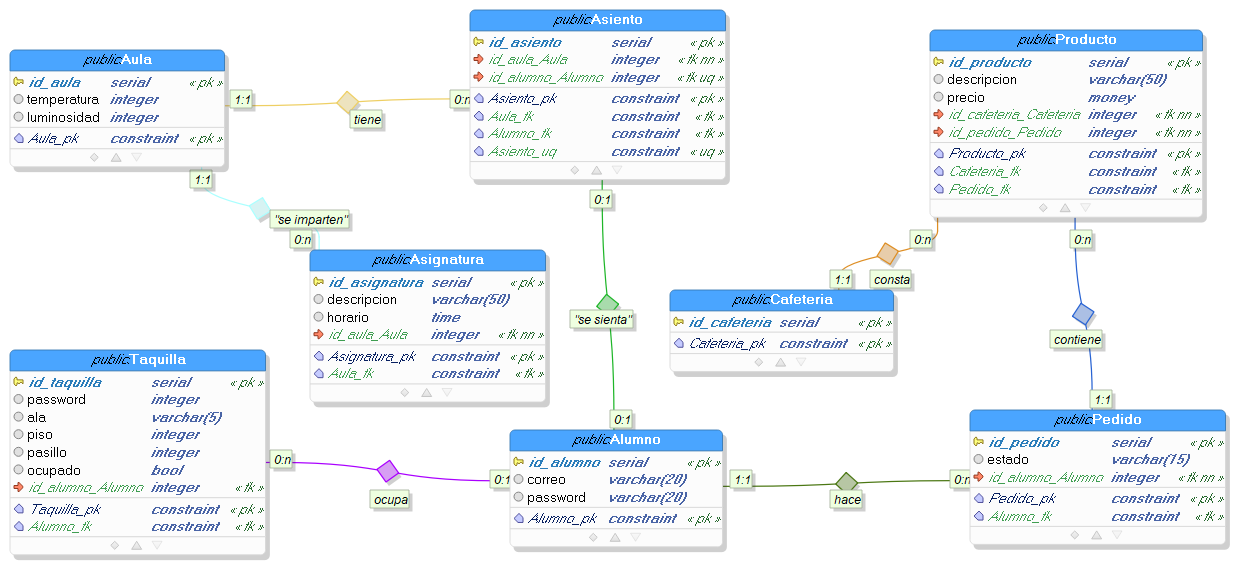
\includegraphics[scale = 0.5]{ImagenBD.png}
    \caption{Primera versión del modelo E/R}
    \label{fig:Figura4}
\end{figure}
\newpage
\section{Modelo E/R: Versión 2}
En esta versión podemos observar un modelo mucho más avanzado. Los principales cambios con respecto a la versión inicial son:

\begin{itemize}
    \item Creación de una nueva tabla \textit{Horario} para contemplar que una asignatura se pueda impartir en diferentes tramos horarios y en diferentes días lectivos.
    \item Relación \textit{Asignatura-Alumno}: dado que esta era una relación \textit{n:m}, se ha normalizado mediante la creación de la tabla \textit{Matricula}.
    \item Creación de una nueva tabla \textit{NFC} que será empleada para guardar el identificador de cada NFC que estará asignado a un pedido.
    \item Modificación de la tabla \textit{Cafetería}: en esta versión decidimos denominarla como \textit{Empleado} puesto que la universidad tiene una única cafetería. Con esta tabla creamos un nuevo rol que será el encargado de preparar los productos para los pedidos.
    \item Relación \textit{Pedido-Producto}: dado que esta era una relación \textit{n:m}, se ha normalizado mediante la creación de la tabla \textit{Pedido\_Producto}.
    \item Añadidas nuevas columnas en la tabla \textit{Aula} como laboratorio, planta, ala, ...
    \item Se ha eliminado la relación \textit{Asignatura-Aula} y se han añadido dos nuevas relaciones: \textit{Asignatura-Horario} y \textit{Horario-Aula}.
\end{itemize}  

\begin{figure}[H]
    \centering
    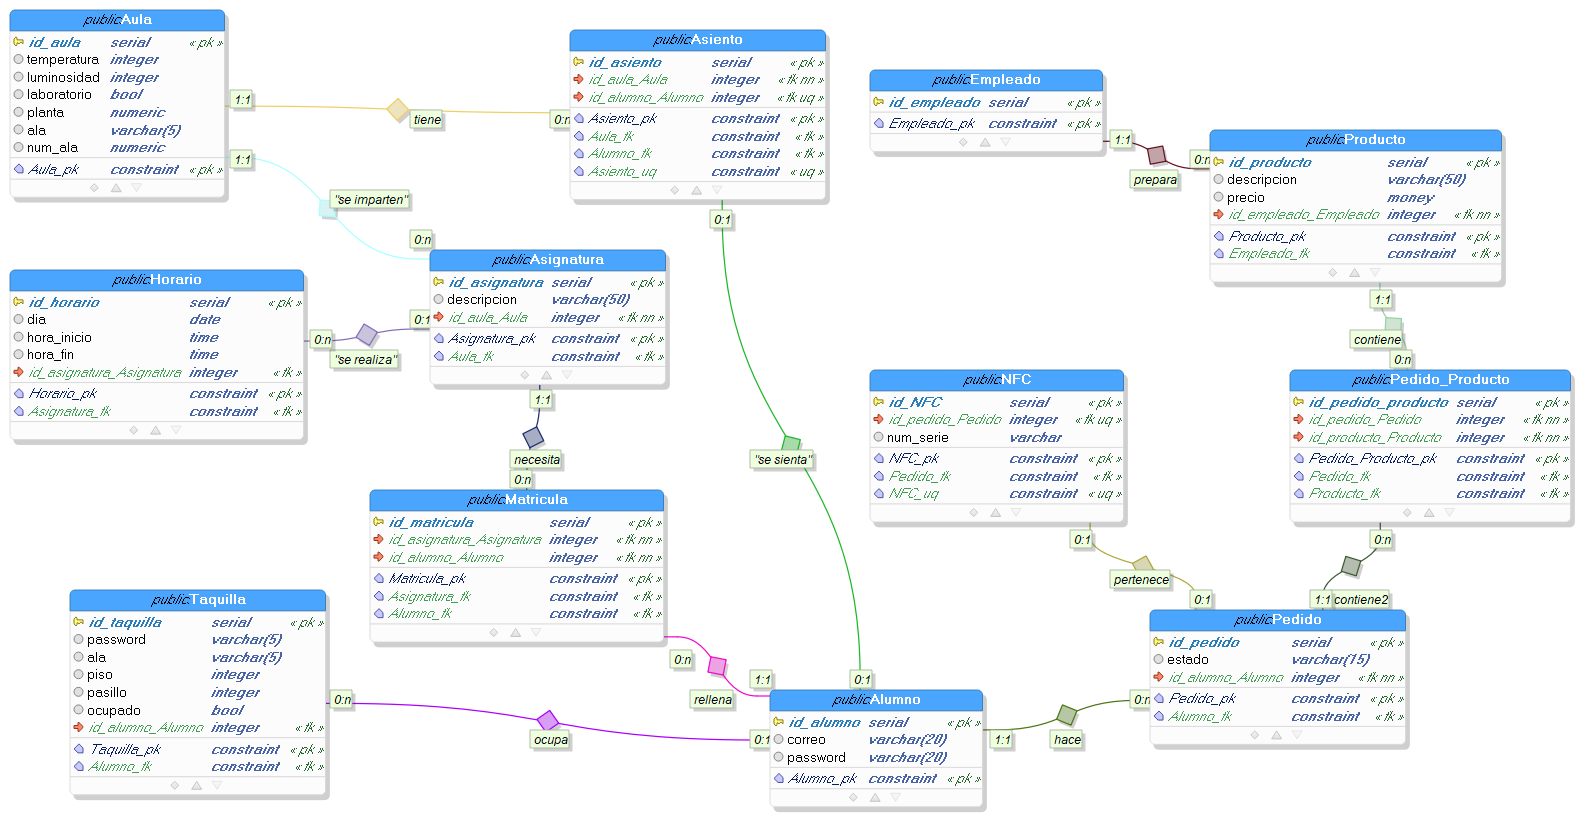
\includegraphics[scale = 0.4]{ImagenBD2.png}
    \caption{Segunda versión del modelo E/R}
    \label{fig:Figura3.4.2}
\end{figure}

\section{Modelo E/R: Versión 3}
Esta es la última y la definitiva versión del modelo E/R del sistema. Los principales cambios con respecto a la anterior versión son:
\begin{itemize}
    \item Se ha añadido una nueva tabla \textit{Histórico\_Aula}: en esta tabla se almacena la temperatura a la que se encontraba el aula así como el tiempo que tarda en llegar a la temperatura óptima.
    \item Añadidas nuevas columnas en \textit{Producto}: se ha añadido tanto un breve detalle del producto como una imagen de este.
\end{itemize} 

\begin{figure}[H]
    \centering
    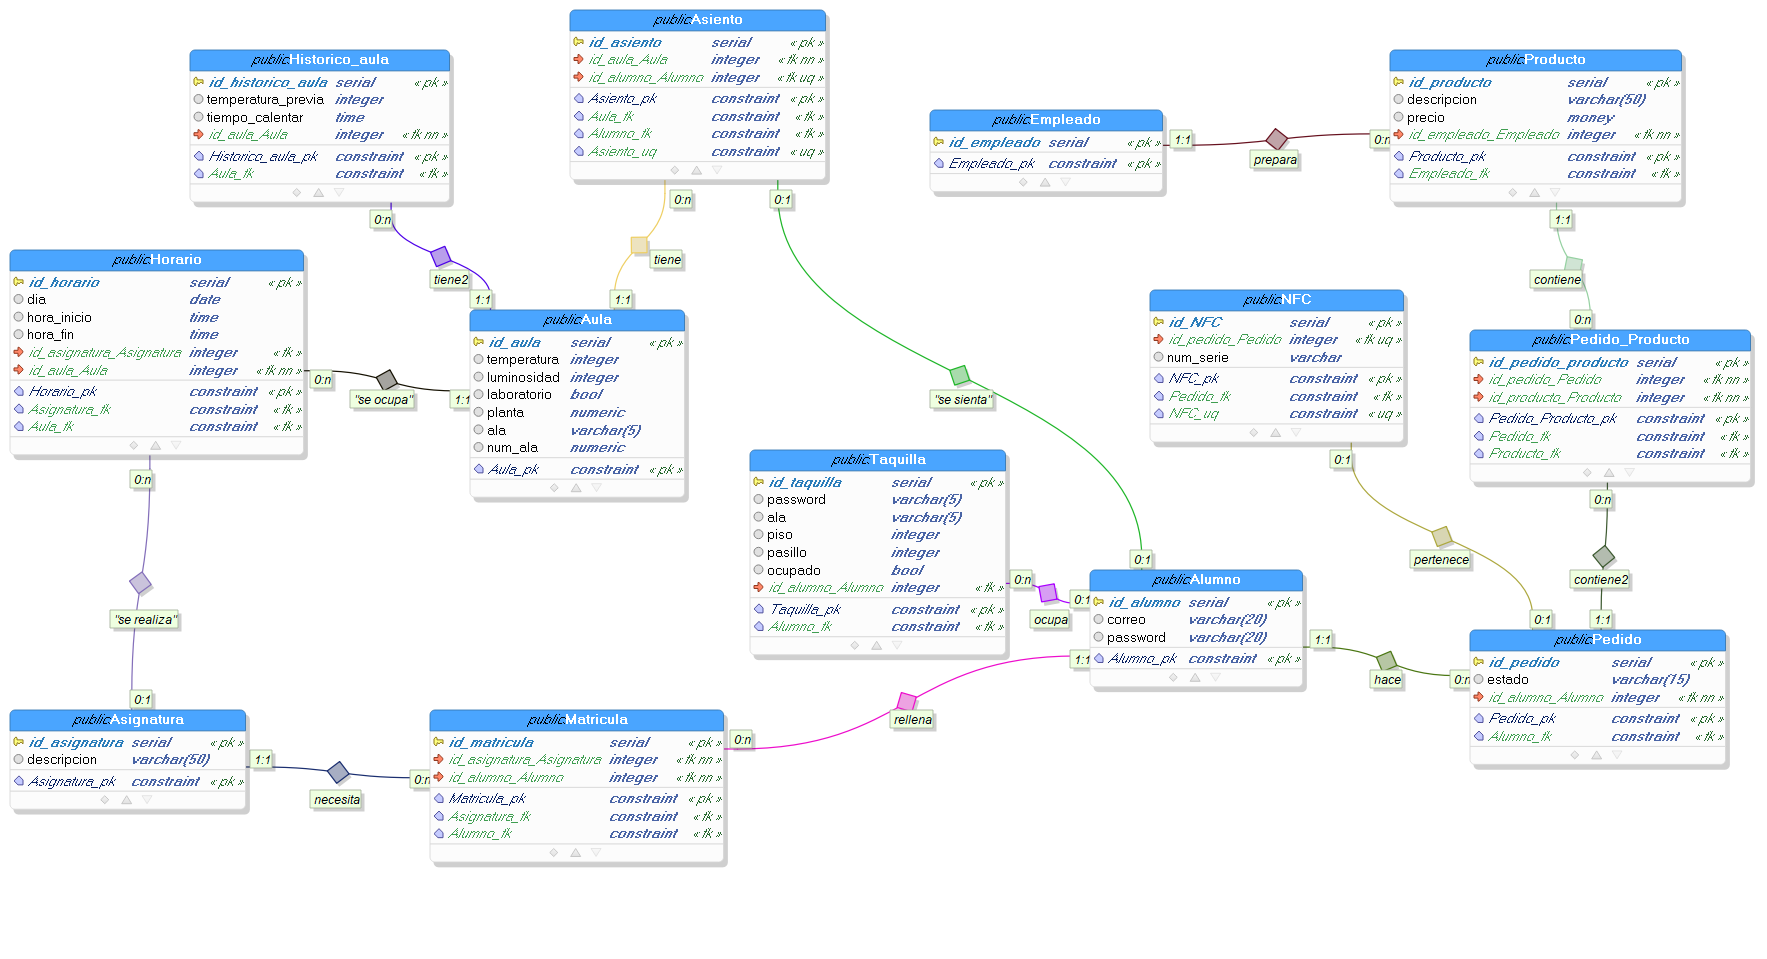
\includegraphics[scale = 0.35]{ImagenBD3.png}
    \caption{Última versión del modelo E/R}
    \label{fig:Figura3.4.3}
\end{figure}

\section{Esquema de tablas}
A continuación, detallaremos las distintas tablas del modelo E/R así como sus distintos atributos:
\begin{itemize}
    \item\textbf{Alumno}: son los principales usuarios de nuestro sistema. Dentro de esta tabla almacenaremos:
    \begin{itemize}
        \item \textbf{Id\_alumno}: se trata de un serial que nos permitirá identificar a cada alumno ya que es \textit{PRIMARY\_KEY}.
        \item \textbf{Correo}: se trata del propio correo electrónico del alumno.
        \item \textbf{Password}: se trata de la contraseña asociada al correo electrónico del alumno.
        \\\\\\
    \end{itemize}
    
    \item\textbf{Taquilla}: en esta tabla se almacenarán las principales características de cada una de las taquillas de la universidad. Estas características son:
    
    \begin{itemize}
        \item\textbf{Id\_taquilla}: se trata de un serial que nos permitirá identificar cada taquilla ya que es \textit{PRIMARY\_KEY}.
        \item \textbf{Password}: se trata de la contraseña asociada a la taquilla para que esta se pueda abrir correctamente.
        \item \textbf{Ala}: dado que la escuela se divide en distintas alas (Este, Norte, Oeste y Sur), en este campo almacenaremos la ubicación.
        \item \textbf{Piso}: almacenaremos también el piso en el que se encuentra cada taquilla.
        \item \textbf{Pasillo}: en cada ala hay dos pasillos distintos, por lo que almacenaremos el pasillo en el que se encuentra la taquilla.
        \item \textbf{Ocupado}: se trata de un valor booleano que nos indicará si dicha taquilla pertenece o no a un alumno.
        \item \textbf{Id\_alumno\_alumno}: como las taquillas se relacionan con los alumnos, en caso de que una taquilla este ocupada se almacenará el id del alumno que la ha reservado.
        \\
    \end{itemize}
    \item \textbf{Aula}: en esta tabla se almacenarán las principales características de cada aula. Estas son:
    \begin{itemize}
        \item\textbf{Id\_aula}: se trata de un serial que nos permitirá identificar cada aula ya que es \textit{PRIMARY\_KEY}.
        \item \textbf{Temperatura}: almacenaremos la temperatura de cada aula gracias a un sensor de temperatura.
        \item \textbf{Luminosidad}: al igual que la temperatura, también se almacenará la luminosidad del aula.
        \item \textbf{Laboratorio}: almacenaremos si el aula es o no un laboratorio.
        \item \textbf{Planta}: al igual que en las taquillas, almacenaremos en que planta se encuentra el aula.
        \item \textbf{Ala}: dado que la escuela se divide en distintas alas (Este, Norte, Oeste y Sur), en este campo almacenaremos la ubicación.
        \item \textbf{Num\_ala}: almacenaremos cuál es el número de aula.
        \\
    \end{itemize} 
    \item  \textbf{Historico\_Aula}: para poder saber cuánto tiempo se necesita para que la temperatura de un aula sea la óptima, hemos creado esta tabla. En ella se guardarán las siguientes características
    \begin{itemize}
        \item\textbf{Id\_Historico\_Aula}: se trata de un serial que nos permitirá identificar cada histórico de un aula ya que es \textit{PRIMARY\_KEY}.
        \item \textbf{Temperatura\_previa}: se almacenará la temperatura a la que se encontraba el aula antes de haber llegado a su temperatura óptima.
        \item \textbf{Tiempo\_calentar}: se almacenará también el tiempo que se ha tardado en llegar desde la temperatura previa a la temperatura óptima.
        \item \textbf{Id\_aula\_aula}: como los históricos se relacionan con las aulas, almacenamos el id del aula donde se ha realizado un cambio de temperatura.
        \\
    \end{itemize} 
    \item  \textbf{Asignatura}: dado que en la universidad se imparten distintas asignaturas, almacenaremos las siguientes características:
    \begin{itemize}
        \item\textbf{Id\_asignatura}: se trata de un serial que nos permitirá identificar cada asignatura ya que es \textit{PRIMARY\_KEY}.
        \item \textbf{Descripción}: se trata del nombre de la asignatura impartida.
        \\
    \end{itemize} 
    \item  \textbf{Horario}: para saber cuándo se ocupa una determinada aula, usaremos los horarios. En esta tabla se almacenan:
    \begin{itemize}
        \item\textbf{Id\_horario}: se trata de un serial que nos permitirá identificar cada horario ya que es \textit{PRIMARY\_KEY}.
        \item \textbf{Día}: almacenaremos el día en el que se imparte una asignatura.
        \item \textbf{Hora\_inicio}: almacenaremos la hora en la que empieza una asignatura.
        \item \textbf{Hora\_fin}: almacenaremos la hora en la que finaliza una asignatura.
        \item \textbf{Id\_asignatura\_asignatura}: como los horarios se relacionan con las asignaturas, almacenamos el id de la asignatura que se imparte en dicho horario.
        \item \textbf{Id\_aula\_aula}: como los horarios se relacionan con las aulas, almacenamos el id del aula donde se imparte la asignatura en dicho horario.
        \\
    \end{itemize} 
    \item  \textbf{Empleado}: para la implementación de la parte de la cafetería hemos creado un usuario que se encarga de preparar los distintos productos. Almacenamos en esta tabla la siguiente característica:
    \begin{itemize}
        \item\textbf{Id\_empleado}: se trata de un serial que nos permitirá identificar cada empleado de la cafetería ya que es \textit{PRIMARY\_KEY}.
        \\
    \end{itemize} 
    \item  \textbf{Producto}: la cafetería ofrece diversos productos que se encuentran almacenados en la base de datos en esta tabla. Las características de cada producto son:
    \begin{itemize}
        \item\textbf{Id\_producto}: se trata de un serial que nos permitirá identificar cada producto ya que es \textit{PRIMARY\_KEY}.
        \item \textbf{Descripción}: se almacenará el nombre de cada producto que se ofrece en la cafetería.
        \item \textbf{Precio}: se almacenará el precio por unidad de cada producto.
        \item \textbf{Id\_empleado\_empleado}: como los productos se relacionan con los empleados de la cafetería, almacenamos el id del empleado que prepara cada producto.
        \\\\\\
    \end{itemize} 
    \item \textbf{Pedido}: al poder realizar un pedido de la cafetería desde la página web, almacenaremos los siguientes datos en esta tabla:
    \begin{itemize}
        \item\textbf{Id\_pedido}: se trata de un serial que nos permitirá identificar cada pedido ya que es \textit{PRIMARY\_KEY}.
        \item \textbf{Estado}: para saber si nuestro pedido está listo observaremos este valor:
        \begin{itemize}
            \item \textbf{0}: nos indica que la petición del pedido ha sido recibida y está pendiente de aprobarse.
            \item \textbf{1}: nos indica que el pedido ha sido aceptado y se está preparando en la cocina.
            \item \textbf{2}: nos indica que el pedido ha sido preparado correctamente y está listo para ser recogido.
            \item \textbf{3}: nos indica que el pedido ha sido recogido y por tanto se está consumiendo.
            \item \textbf{4}: nos indica que el pedido ha sido consumido y por tanto finalizado.
        \end{itemize}
        \item \textbf{Id\_alumno\_alumno}: como los pedidos se relacionan con los alumnos, se almacenará el id del alumno que ha realizado el pedido. 
    \\
    \end{itemize} 
    \item  \textbf{Pedido\_Producto}: esta tabla, tal y como se ha explicado en el modelo E/R, surge porque la relación entre \textit{Pedido} y \textit{Producto} es \textit{n:m}. Esta tabla se compone de:
    \begin{itemize}
        \item\textbf{Id\_pedido\_producto}: se trata de un serial que nos permitirá identificar cada pedido\_producto ya que es \textit{PRIMARY\_KEY}.
        \item\textbf{Id\_pedido\_pedido}: nos permitirá identificar el pedido.
        \item\textbf{Id\_producto\_producto}: nos permitirá identificar el producto.
        \\
    \end{itemize} 
    \item  \textbf{NFC}: en la cafetería emplearemos los NFCs para poder recoger los pedidos. Esta tabla se compone de:
    \begin{itemize}
        \item\textbf{Id\_NFC}: se trata de un serial que nos permitirá identificar cada NFC ya que es \textit{PRIMARY\_KEY}.
        \item\textbf{Id\_pedido\_pedido}: nos permitirá identificar el pedido.
        \item\textbf{Num\_serie}: cada NFC lleva asociado un número de serie por lo que almacenaremos dicho valor.
    \\
    \end{itemize} 
\end{itemize} 

\section{Tablas extra}
Se puede observar que las tablas \textit{Asiento} y \textit{Matrícula} no se usan en el sistema actual. Esto se debe a que nuestro proyecto es escalable y serían futuras mejoras. Por ejemplo, la tabla \textit{Asiento} almacenaría gracias a NFC donde está situado un alumno en el Aula.
\newpage
\section{Vistas}
Además de las tablas mencionadas en los apartados anteriores, dentro de la base de datos podemos observar distintas vistas:
\begin{itemize}
    \item \textbf{Vista asignaturas}: dentro de esta vista podremos observar las distintas características de una asignatura así como la clase donde se imparte y en qué horario.
    \begin{figure}[H]
        \centering
        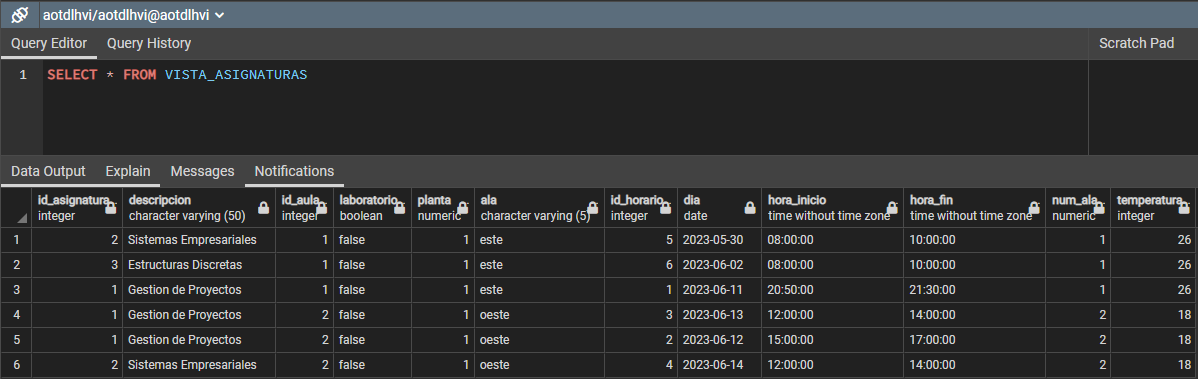
\includegraphics[scale = 0.55]{Vista_asignaturas.png}
        \caption{Vista asignaturas}
        \label{fig:Figura}
    \end{figure}
    
    \item \textbf{Vista pedido estrella}: dentro de esta vista podremos observar los distintos productos que se encuentran en los pedidos junto a la descripción de estos pedidos y al identificador del alumno.
    \begin{figure}[H]
        \centering
        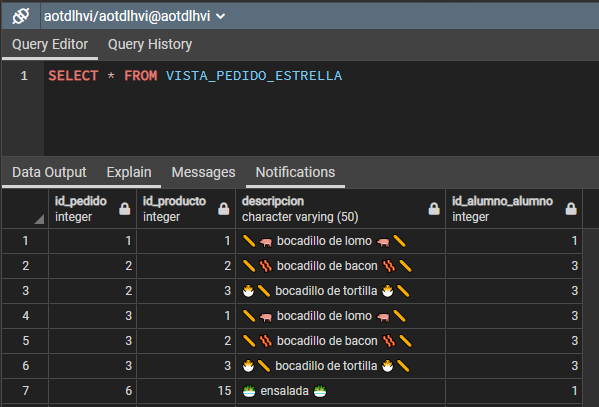
\includegraphics[scale = 0.75]{Vista_pedido_estrella.png}
        \caption{Vista pedido estrella}
        \label{fig:Figura}
    \end{figure}
    \newpage
    \item \textbf{Vista pedidos}: dentro de esta vista podremos observar todos los productos que ha ordenado un alumno en un único pedido.
    \begin{figure}[H]
        \centering
        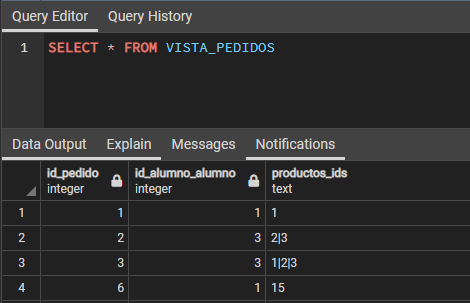
\includegraphics[scale = 0.65]{Vista_pedidos.png}
        \caption{Vista pedidos}
        \label{fig:Figura}
    \end{figure}
    
    \item \textbf{Vista resumen aula}: dentro de esta vista obtendremos cuál es la próxima asignatura que se imparte en un aula y si es necesario actuar en ella para llegar a conseguir la temperatura óptima antes de que empiece la asignatura.
    \begin{figure}[H]
        \centering
        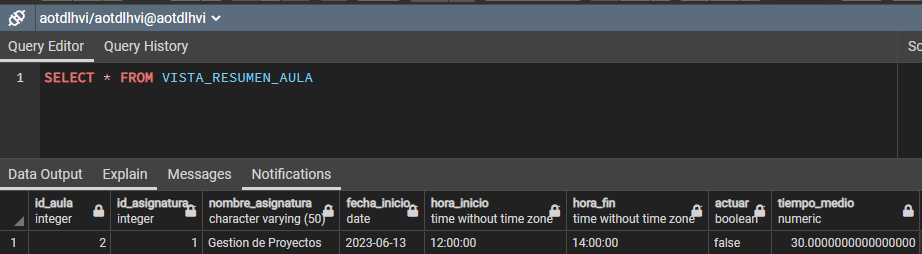
\includegraphics[scale = 0.65]{Vista_resumen_aula.png}
        \caption{Vista resumen aula}
        \label{fig:Figura}
    \end{figure}
\end{itemize}

\section{Instalación y configuración}
En cuanto a la instalación y configuración de la propia base de datos, hemos optado por obtener una online gratuita hosteada de manera remota. Se trata de una base de datos en PostgreSQL que permite 5 conexiones simultáneas.
\\\\
Para acceder a ella hemos optado por utilizar un gestor de bases de datos. En nuestro caso hemos utilizado dos diferentes, dependiendo del miembro del grupo: \textit{pgAdmin4} y \textit{Dbeaver}. Dentro del gestor, crearemos un servidor con las credenciales que hemos obtenido. Una vez verificadas, podremos acceder a nuestra base de datos sin problemas.
\\\\
Para insertar las distintas tablas que hemos mencionado anteriormente usaremos el código SQL que podemos exportar desde \textit{pgModeler}. Cuando tengamos este código lo copiaremos y pegaremos en la propia base de datos. Una vez insertadas todas las tablas hemos añadido algunos datos de prueba que se encuentran en el fichero \textit{DatosBD3.sql}.


\chapter{Desarrollo de la API}
Como se ha detallado anteriormente, este apartado ha sido desarrollado por completo utilizando el \textit{framework} de \textit{FastApi} para el lenguaje \textit{Python}. Un desarrollo de un \textit{Backend} complejo y sofisticado siempre es una tarea de alta dificultad, sin embargo; gracias a utilizar este \textit{framework}, nuestro trabajo se ha simplificado y acelerado en gran medida.
\\
A continuación se detallarán aspectos importantes a destacar de la implementación realizada.
\section{Estructura clara y organizada}
Desde el inicio del proyecto, hicimos hincapié en la importancia de contar con una estructura de código clara y organizada, que permitiera localizar rápidamente cualquier aspecto del mismo.
\\

En este contexto, la implementación adoptada se basa en un archivo principal denominado \texttt{main.py}, el cual contiene la aplicación \textit{FastAPI}. A este archivo se agregan todos los nodos terminales que se encuentran en la carpeta \textit{endpoints}. Estos endpoints se encuentran distribuidos en varios archivos \textit{.py}, clasificados de acuerdo con el aspecto de la \textit{API} que manejan. Por ejemplo, se pueden encontrar archivos como \textit{taquillas.py}, \textit{productos.py}, entre otros.
\\

Además de la organización de los endpoints, esta implementación también proporciona una forma sencilla de agregar todos los archivos necesarios para mostrar la interfaz de usuario (\emph{frontend}). Esto implica que la estructura del proyecto permite incorporar de manera eficiente los archivos relevantes para la interfaz de usuario, facilitando así su desarrollo y mantenimiento.
\\

A continuación se muestra un diagrama de la estructura utilizada:
\begin{figure}[H]
    \centering
\begin{tikzpicture}[
  level 1/.style={sibling distance=60mm},
  level 2/.style={sibling distance=30mm},
  level 3/.style={sibling distance=20mm}
]
\node {main.py}
  child {node {endpoints}
    child {node {taquillas.py}}
    child {node {productos.py}}
    child {node {sesion.py}}
    child {node {aulas.py}}
    child {node {...}}
  };
\end{tikzpicture}
\caption{Diagrama de la estructura del proyecto}
\label{fig:arbol_estructura}
\end{figure}

\section{Manejo de errores}
Se ha implementado un sistema que permite lanzar errores que se le pueden mostrar al cliente de manera detallada; donde se le muestra el código de estado de la llamada \textit{HTTP}, junto con un mensaje detallando la causa del problema. La mayor complicación ha sido implementar el sistema haciendo que en el momento en el que se quiera mandar dicha respuesta al cliente, se interrumpa toda la ejecución y se devuelva únicamente el error especificado.

\section{Impresión interrumpida}
El método de depuración \texttt{printerrupt()} ofrece una solución eficiente para la depuración de nuestra \textit{API}.

El método \texttt{printerrupt()} permite interrumpir rápidamente la ejecución del programa y devuelve al cliente una cadena de texto plano especificada como argumento. Esta función resulta especialmente útil en situaciones en las que es difícil determinar la causa de un error en un momento determinado. Al proporcionar una forma de interrumpir la ejecución y obtener información en forma de texto plano, este método simplifica el proceso de identificación y resolución de cualquier tipo de error o fallo (\emph{bug}).

El uso de \texttt{printerrupt()} permite una depuración más eficiente al proporcionar una herramienta que ayuda a acotar el problema en cuestión. Al interrumpir la ejecución y enviar una respuesta al cliente, se facilita la identificación de puntos críticos en el código y se agiliza la solución de problemas.
\section{Utilidades para la base de datos}
Se han creado una serie de métodos que facilitan muy notoriamente el manejo de las conexiones a la base de datos donde se almacenan todos los datos.

Entre estos métodos destacan:
\begin{itemize}
    \item \texttt{realizar\_insercion}:
    \\
    Realiza la inserción de datos en una tabla de la base de datos, simplemente pasándole como argumentos el nombre de la tabla y un diccionario (\textit{JSON}) cuyos campos serán las columnas de la tabla. El método inteligentemente realiza una serie de verificaciones previas para asegurar que todo funcionará correctamente y cuenta con un manejo de errores detallado. A continuación, se muestran los pasos que sigue este método:

\begin{enumerate}
    \item Establece una conexión a la base de datos utilizando una función llamada \texttt{get\_connection()}.
    
    \item Verifica si la tabla especificada existe en la base de datos. Para ello, ejecuta una consulta de selección limitada a un solo registro en la tabla. Si la consulta arroja un error, se interpreta como que la tabla no existe y se genera un mensaje de error.
    
    \item Determina el nombre de la columna que actúa como clave primaria en la tabla. Esto se hace consultando el esquema de la base de datos y buscando la columna que tiene la restricción de ``\textit{PRIMARY KEY}".
    
    \item Verifica que la columna de la clave primaria no se haya proporcionado en el diccionario de datos o que su valor sea `\textit{None}`. Si se proporciona o su valor no es `\textit{None}`, se genera un mensaje de error. Los IDs de la base de datos implementada son del tipo Serial y se establecen automáticamente, por lo que no se deben enviar a la hora de realizar inserciones en la base de datos.
    
    \item Obtiene los nombres de todas las columnas de la tabla desde el esquema de la base de datos.
    
    \item Revisa que todas las columnas enviadas en el diccionario de datos existan en la tabla. Si alguna columna no existe, se genera un mensaje de error.
    
    \item Elimina las columnas de la lista que no están presentes en el diccionario de datos. Esto asegura que solo se inserten los valores para las columnas proporcionadas.
    % Aquellos que no estén se insertarán como nulos, siempre y cuando la tabla lo permita.
    
    \item Verifica que no falten campos requeridos que no pueden ser nulos en la base de datos. Esto se hace consultando los campos no nulos de la tabla y comparándolos con los campos proporcionados en el diccionario de datos. Si falta algún campo requerido, se genera un mensaje de error.
    
    \item Agrega `\textit{None}` como valor para las columnas que no están presentes en el diccionario de datos. Esto garantiza que se inserten `\textit{NULL}` en esas columnas.
    
    \item Construye una consulta de inserción automáticamente utilizando el nombre de la tabla y las columnas correspondientes. La columna de la clave primaria se omite en esta consulta por lo que se mencionó anteriormente.
    
    \item Ejecuta la consulta de inserción en la base de datos utilizando una función llamada `\texttt{insertar\_datos\_conexion()}`. Si ocurre un error de integridad debido a una violación de clave primaria, se genera un mensaje de error. Realmente, no debería haberlo nunca, pero pese a ello, se maneja dicho error.
    
    \item Obtiene el valor de la clave primaria del nuevo registro insertado utilizando una consulta que obtiene el valor actual de la secuencia de la clave primaria.
    
    \item Cierra la conexión a la base de datos.
    
    \item Retorna el valor de la clave primaria del nuevo registro insertado.
\end{enumerate}
En resumen, este método se encarga de realizar la inserción de datos en una tabla de una base de datos creando inteligentemente una consulta procesada. Esto se realiza verificando la existencia de la tabla, la validez de los datos proporcionados, la presencia de campos requeridos y la integridad de la clave primaria. Además, se encarga de manejar los mensajes de error y retorna el valor de la clave primaria del nuevo registro.

\item \texttt{realizar\_actualizacion}
Este método, de manera similar al anterior, se encarga de realizar una actualización en una tabla de una base de datos recibiendo únicamente el nombre de la tabla, el id del registro y un diccionario con aquellos campos que se deseen actualizar. Este método realiza la actualización tras verificar y manejar cualquier tipo de problema. A continuación, se detallan los pasos que sigue este método:

\begin{enumerate}
    \item Establece una conexión a la base de datos utilizando una función llamada `\texttt{get\_connection()}`.
    \item Verifica si la tabla especificada existe en la base de datos. Para ello, ejecuta una consulta de selección limitada a un solo registro en la tabla. Si la consulta arroja un error, se interpreta como que la tabla no existe y se genera un mensaje de error.
    \item Determina el nombre de la columna que actúa como clave primaria en la tabla. Esto se hace consultando el esquema de la base de datos y buscando la columna que tiene la restricción de "PRIMARY KEY".
    \item Verifica que la columna de la clave primaria no se haya enviado en el diccionario de datos y que el parámetro `id` no sea `None`. Si se envía la columna o `id` es `None`, se genera un mensaje de error.
    \item Obtiene los nombres de todas las columnas de la tabla desde el esquema de la base de datos.
    \item Verifica que exista un registro en la tabla con el valor de clave primaria especificado en el parámetro `id`. Si no existe un registro con ese valor de clave primaria, se genera un mensaje de error.
    \item Verifica que todas las columnas enviadas en el diccionario de datos existan en la tabla. Si alguna columna no existe, se genera un mensaje de error.
    \item Verifica que los campos con valor `None` puedan ser nulos en la base de datos. Esto se hace consultando los campos no nulos de la tabla y comparándolos con los campos y sus valores proporcionados en el diccionario de datos. Si se intenta asignar un valor `None` a un campo no nulo, se genera un mensaje de error.
    \item Construye la consulta de actualización y los valores a actualizar. Las columnas y sus respectivos valores se obtienen del diccionario de datos, excluyendo la columna de la clave primaria y las columnas que tienen un valor `None`. La consulta de actualización se construye utilizando la sintaxis SQL adecuada.
    \item Ejecuta la consulta de actualización en la base de datos utilizando una función llamada `\texttt{actualizar\_datos\_conexion()}`. Si ocurre un error de integridad debido a una violación de clave primaria, se genera un mensaje de error.
    \item Cierra la conexión a la base de datos.
    \item Retorna el valor del parámetro `id`.
\end{enumerate}

En resumen, este método se encarga de realizar una actualización en una tabla de una base de datos, verificando la existencia de la tabla, la validez de los datos proporcionados, la presencia de la clave primaria y las columnas, y la posibilidad de asignar valores `\textit{None}` a campos nulos. Además, se encarga de manejar los mensajes de error y retorna el valor del parámetro `id`.
\end{itemize}

\section{Endpoints}
Como se ha mencionado en apartados anteriores, los \textit{endpoints} han sido organizados de manera categórica dentro de diversos ficheros. Nuestros endpoints se han distinguido en las siguientes categorías
\begin{itemize}
    \item Sesión\\
    Dentro del fichero \textit{sesion.py} se pueden encontrar los \textit{endpoints} relacionados con el inicio de sesión y registro de usuarios en la plataforma. Un usuario al ser registrado, recibe un email de bienvenida.
    \item Páginas HTML\\
    Dentro del fichero \textit{paginasHTML.py} se alojan todos los endpoints que retornan las páginas \textit{HTML} junto con su hoja de estilos \textit{CSS} y código \textit{JavaScript} asociado. Es una manera simple y organizada de conectar el \textit{FrontEnd} al \textit{BackEnd}.
    \item Taquillas\\
    En el fichero \textit{taquillas.py} podemos encontrar todos los nodos terminales relacionados con la gestión de taquillas.
    Entre dichos endpoints encontramos:
    \begin{itemize}
        \item \textcolor{ForestGreen}{\texttt{GET}} \textit{Lista Taquillas}\\
        Retorna un listado de todas las taquillas del sistema.\\
        Permite realizar un filtrado según el ala, el piso y el pasillo de la taquilla.
        Localizado en: \texttt{(host)/taquillas}
        \item \textcolor{ForestGreen}{\texttt{GET}} \textit{Detalle taquilla}\\
        Retorna la información completa y detallada de una taquilla en específico.\\
        Para ello recibe como argumento el id de la taquilla deseada como path parameter.\\
        Localizado en: \texttt{(host)/taquillas/\{id\_taquilla\}}
        \item \textcolor{YellowOrange}{\texttt{POST}} \textit{Insertar taquilla}\\
        Permite insertar una nueva taquilla en el sistema con la información que se envíe en el body de la solicitud.
        \\Localizado en: \texttt{(host)/taquillas}
        \\Ejemplo de cuerpo de la solicitud:
        \begin{verbatim}
            {
                "ala": "este",
                "pasillo": 2,
                "piso": 2
            }
        \end{verbatim}
        \item \textcolor{SkyBlue}{\texttt{PUT}} \textit{Reservar taquilla}\\
        Este endpoint permite reservar una taquilla a partir de una taquilla y un alumno y genera una contraseña.\\
        Recibe como parámetro el \texttt{id\_taquilla} de la taquilla deseada y la información del alumno en el cuerpo de la solicitud.\\
        Localizado en: \texttt{(host)/taquillas/reservar/\{id\_taquilla\}}\\
       
        
        \item \textcolor{SkyBlue}{\texttt{PUT}} \textit{Cancelar taquilla}\\
        Este endpoint cancela la reserva o la asignación de una taquilla a un alumno.\\
        Recibe como parámetros el \texttt{id\_taquilla} y el \texttt{id\_alumno} de la taquilla y el alumno respectivamente.\\
        Localizado en: \texttt{(host)/taquillas/cancelar/\{id\_taquilla\}/\{id\_alumno\}}
                \\Ejemplo de cuerpo de la solicitud:
        \begin{verbatim}
        {
          "id_alumno": 7
        }
        \end{verbatim}
        
        
        
        \item \textcolor{ForestGreen}{\texttt{GET}} \textit{Obtener taquilla reservada}\\
        Este endpoint devuelve el ID de la taquilla reservada por un alumno específico.\\
        Recibe como parámetro el \texttt{id\_alumno} del alumno.\\
        Localizado en: \texttt{(host)/taquilla/Alumno/\{id\_alumno\}}
        \item \textcolor{YellowOrange}{\texttt{POST}} \textit{Abrir taquilla}\\
        Este endpoint permite abrir una taquilla a partir de su ID y una contraseña.\\
        Recibe como parámetro el \texttt{id\_taquilla} de la taquilla deseada y la contraseña en el cuerpo de la solicitud.\\
        Localizado en: \texttt{(host)/taquillas/\{id\_taquilla\}}\\
        Ejemplo de cuerpo de la solicitud:
        \begin{verbatim}
        {
          "password": "contraseña"
        }
        \end{verbatim}
        
    \end{itemize}
    \item Aulas\\
Todos los endpoints relacionados con la gestión de las aulas se pueden encontrar en \textit{aulas.py}. Entre dichos endpoints encontramos:
\begin{itemize}
    \item \textcolor{ForestGreen}{\texttt{GET}} \textit{Lista Aulas}\\
    Retorna un listado de todas las aulas de la Escuela Politécnica Superior. Permite también realizar una búsqueda filtrada según el piso del aula, su tipo (Laboratorio o Aula de teoría), ala (Norte, Sur, Este y Oeste)... Dicho filtro se realiza a partir de los query params recibidos.\\
    Localizado en: \texttt{(host)/aulas}
    
    \item \textcolor{ForestGreen}{\texttt{GET}} \textit{Info aula}\\
    Retorna la información completa y detallada de un aula en concreto.\\
    Para ello recibe como argumento el id del aula deseada como path parameter.\\
    Localizado en: \texttt{(host)/aulas/\{id\_aula\}}
        
    \item \textcolor{YellowOrange}{\texttt{POST}} \textit{Insertar aula}\\
    Permite insertar una nueva aula en el sistema con la información que se envíe en el body de la solicitud.\\
    Localizado en: \texttt{(host)/aulas}
        \\Ejemplo de cuerpo de la solicitud:
        \begin{verbatim}
        {
            "temperatura": 23,
            "luminosidad": 40,
            "laboratorio": true,
            "planta": "2",
            "ala": "Sur",
            "num_ala": 3
        }
        \end{verbatim}
        
    \item \textcolor{SkyBlue}{\texttt{PUT}} \textit{Actualizar aula}\\
    Permite actualizar los valores de un aula concreta del sistema con la información que se envíe en el body de la solicitud. Este endpoint es utilizado por parte del Arduino para actualizar valores como la temperatura en tiempo real.\\
    Localizado en: \texttt{(host)/aulas/\{id\_aula\}}
        \\Ejemplo de cuerpo de la solicitud:
        \begin{verbatim}
        {
            "temperatura": 23,
            "luminosidad": 40,
            "laboratorio": true,
            "planta": "2",
            "ala": "Sur",
            "num_ala": 3
        }
        \end{verbatim}
        
    \item \textcolor{ForestGreen}{\texttt{GET}} \textit{Asignaturas de aula}\\
    Obtiene las asignaturas que se imparten en un aula específica.\\
    Recibe como parámetro el \texttt{id\_aula} del aula deseada.\\
    Localizado en: \texttt{(host)/aulas/asignaturas/\{id\_aula\}}
    
    \item \textcolor{ForestGreen}{\texttt{GET}} \textit{Disponibilidad de aula}\\
    Se utiliza para saber si un aula está en uso en los próximos minutos. Principalmente usado por el Arduino para saber si debe encender o apagar el aire acondicionado.\\
    Recibe como parámetro el \texttt{id\_aula} del aula deseada.\\
    Localizado en: \texttt{(host)/aulas/disponibilidad/\{id\_aula\}}
    
    \item \textcolor{ForestGreen}{\texttt{GET}} \textit{Horario de aula}\\
    Obtiene el horario de un aula en específico.\\
    Recibe como parámetro el \texttt{id\_horario} del horario deseado.\\
    Localizado en: \texttt{(host)/aulas/horarios/\{id\_horario\}}
    
    \item \textcolor{YellowOrange}{\texttt{POST}} \textit{Insertar horario}\\
    Permite insertar un nuevo horario de clase en el sistema con la información que se envíe en el body de la solicitud.\\
    Localizado en: \texttt{(host)/aulas/horarios}
            \\Ejemplo de cuerpo de la solicitud:
        \begin{verbatim}
        {
             "dia": "2023/06/02",
             "hora_inicio": "8:00",
             "hora_fin": "10:00",
             "id_asignatura_asignatura": 3,
             "id_aula_aula": 1
         }
        \end{verbatim}
        
    \item \textcolor{ForestGreen}{\texttt{GET}} \textit{Climatizar aula}\\
    Se encarga de decir si es el momento adecuado para climatizar un aula o no. Esto se realiza de manera inteligente, pues basándose en los datos de las climatizaciones más recientes de ese aula, se estima el tiempo que puede tardar un aula en obtener las condiciones ideales. Teniendo en cuenta ese tiempo y sabiendo cuándo empezará la próxima clase, se devolverá true (para señalar que se debe climatizar el aula) o un error 400 (para señalizar lo opuesto). Realizando gestiones de temperatura de esta manera se reduce en gran medida el consumo de energía para este proceso y se sigue asegurando una temperatura ideal.\\
    Localizado en: \texttt{(host)/aulas/\{id\_aula\}/climatizar}

    \item \textcolor{YellowOrange}{\texttt{POST}} \textit{Insertar histórico}\\
    Tras haber finalizado el proceso de atemperamiento de un aula, el Arduino llamará a este endpoint para anotar la temperatura a la que estaba el aula antes de intervenir, y anotará también el tiempo empleado en adecuar la temperatura. Estos datos serán útiles de cara a mejorar las estimaciones inteligentes explicadas en el endpoint anterior.\\
    Localizado en: \texttt{(host)/aulas/historico}
            \\Ejemplo de cuerpo de la solicitud:
        \begin{verbatim}
      {
          "id_aula_aula":1,
          "temperatura_previa":21,
          "tiempo_calentar":12
      }
        \end{verbatim}
\end{itemize}

    \item Cafetería\\
La implementación de la cafetería se ha distribuido en tres ficheros diferentes:
\begin{itemize}
\item \texttt{productos.py}:
Aquí se encuentra toda la lógica relacionada con los productos de la carta de la cafetería. Cuenta simplemente con dos endpoints:
\begin{itemize}
    \item \textcolor{ForestGreen}{\texttt{GET}} \textit{Productos de la cafetería}\\
    Obtiene todos los productos que están disponibles en la cafetería. Puede filtrar los productos según su nombre, dado un parámetro de búsqueda. Si no se especifica un parámetro de búsqueda, se obtienen todos los productos.\\
    Localizado en: \texttt{(host)/cafeteria/productos}
    \item \textcolor{ForestGreen}{\texttt{GET}} \textit{Detalle de producto}\\
    Detalla toda la información de un producto en específico de la cafetería.\\
    Recibe como parámetro el \texttt{id\_producto} del producto deseado.\\
    Localizado en: \texttt{(host)/cafeteria/productos/\{id\_producto\}}
\end{itemize}

    
    \item \texttt{pedidos.py}
    Aquí se encuentra toda la lógica relacionada con los pedidos de la cafetería. Cuenta con los siguientes endpoints:
    \begin{itemize}

        \item \textcolor{ForestGreen}{\texttt{GET}} \textit{Pedidos de la cafetería}\\
        Obtiene todos los pedidos que se han realizado en la cafetería.\\
        Localizado en: \texttt{(host)/cafeteria/pedidos}
        \item \textcolor{ForestGreen}{\texttt{GET}} \textit{Detalle de pedido}\\
        Detalla toda la información de un pedido en específico de la cafetería.\\
        Recibe como parámetro el \texttt{id\_pedido} del pedido deseado.\\
        Localizado en: \texttt{(host)/cafeteria/pedidos/\{id\_pedido\}}
        \item \textcolor{YellowOrange}{\texttt{POST}} \textit{Insertar pedido}\\
        Este endpoint permite al usuario realizar un pedido.\\
        Localizado en: \texttt{(host)/cafeteria/pedidos}
        \\Ejemplo de cuerpo de la solicitud:
        \begin{verbatim}
            {
                "id_alumno" : 3,
                "productos" : [1,2,3]
            }
        \end{verbatim}

        \item \textcolor{SkyBlue}{\texttt{PUT}} \textit{Actualizar pedido}\\
        Este endpoint permite a la cafetería actualizar un pedido.\\
        Se puede actualizar el estado del pedido.\\
        Localizado en: \texttt{(host)/cafeteria/pedidos/\{id\_pedido\}}
        \\Ejemplo de cuerpo de la solicitud:
        \begin{verbatim}
            
        {
            "id_alumno" : 5,
            "estado" : 2
        }
        \end{verbatim}
        \item \textcolor{ForestGreen}{\texttt{GET}} \textit{Pedido estrella}\\
        Detalla la descripción del producto más pedido.\\
        Recibe como parámetro el \texttt{id\_alumno} del alumno del que se quiere obtener el pedido estrella.\\
        En caso de no especificar el parámetro, se obtendrá el pedido estrella de todos los alumnos.\\
        Se ha implementado de esta manera para poder obtener el pedido estrella de un alumno en concreto, o de todos los alumnos en general.\\
        Localizado en: \texttt{(host)/cafeteria/pedidos/estrella}

    \end{itemize}

    \item \texttt{NFC.py}
    Los NFC cuentan con varios endpoints a destacar. Originalmente iban a tener una funcionalidad que iba a ir más allá de limitarse únicamente a la verificación de pedidos de la cafetería. Desgraciadamente se tuvo que descartar esa idea. Los endpoints a destacar son:
    
\end{itemize}
    
\end{itemize}

\chapter{Diseño e implementación del front-end}
En esta sección, se detalla el diseño y la implementación del front-end de la aplicación web del proyecto. El front-end se encarga de la interfaz de usuario y la interacción con el usuario. Se utilizan tecnologías como HTML, CSS y JavaScript para crear una experiencia visual agradable y funcional. \\

La implementación del front\textendash end se ha realizado utilizando: HTML para la estructura y el contenido de las páginas, CSS para dar estilo y diseño a los elementos visuales, y JavaScript para la interactividad y la lógica de la aplicación en el lado del cliente.
\\

\section{Estructura HTML}
En esta sección se detallan y explican los diferentes elementos y funcionalidades de los archivos HTML utilizados en la implementación del front-end de la aplicación web SmartUni.
\subsection{Página de Inicio de Sesión}
La página de inicio de sesión (index.html) es la primera pantalla que los usuarios ven al acceder a la plataforma SmartUni. Su objetivo es permitir que los usuarios inicien sesión en sus cuentas existentes o se registren como nuevos usuarios. A continuación, se explican los componentes clave de esta página:

\begin{itemize}
    \item El encabezado\textbf{ \textless head\textgreater} del archivo HTML contiene metadatos esenciales, como la codificación de caracteres, la configuración de la vista en los dispositivos y el título de la página. Además, se vincula el archivo main.css para aplicar estilos personalizados a la página. El ícono de SmartUni también se establece a través del enlace a la imagen favicon.png. El archivo index.js se enlaza al final del encabezado y contiene el código JavaScript específico de esta página.

    \item En el cuerpo\textbf{ \textless body\textgreater} de la página, se encuentra el contenido principal contenido dentro del elemento principal \textbf{ \textless main\textgreater}. 

    \begin{itemize}
        \item La página comienza mostrando el logotipo de SmartUni utilizando la etiqueta\textbf{ \textless img\textgreater} con la clase 'logo' para aplicar estilos específicos a la imagen.
        
        \item Se presenta un formulario de inicio de sesión dentro de un contenedor div con la clase 'menu'\textbf{ \textless div class="menu"\textgreater}. El formulario\textbf{ \textless form id="loginForm"\textgreater} solicita al usuario su dirección de correo electrónico y contraseña para autenticarse en la plataforma. Cuando el usuario envía el formulario haciendo clic en el botón 'INICIAR SESIÓN', se ejecuta la función iniciarSesion() definida en el archivo index.js. Los campos de entrada de texto se definen con los elementos\textbf{ \textless input\textgreater}, donde se especifica el tipo de entrada (text o password), y se les asigna un id para identificarlos en el código JavaScript.
        
        \item Si se produce algún error durante el proceso de inicio de sesión, se muestra un mensaje de error utilizando el elemento h3 con la clase 'errorMsg'\textbf{ \textless h3 class=''errorMsg''\textgreater}. Este mensaje se oculta inicialmente estableciendo su estilo de visualización en "none", y el código JavaScript puede mostrarlo si es necesario.
        
        \item  El atributo \textbf{id=''errorInicioSesion''} se utiliza para identificar este elemento en el código JavaScript y aplicar cambios en su estilo.
        
        \item Se proporciona un enlace al formulario de registro para los usuarios que aún no tienen una cuenta. Al hacer clic en el enlace 'REGISTRATE', los usuarios serán redirigidos a la página de registro, ya que el elemento \textbf{\textless a\textgreater} se utiliza como un enlace para redirigir al usuario a la página de registro.
    \end{itemize}
\end{itemize}
Por tanto, la página de inicio de sesión de SmartUni presenta una interfaz sencilla y amigable que permite a los usuarios autenticarse en la plataforma utilizando su correo electrónico y contraseña, ofreciendo la opción de registrarse para los nuevos usuarios.

\subsection{Página de Registro}
El archivo HTML ''registrarse.html'' representa la página de registro en la aplicación SmartUni. Esta página proporciona un formulario para que los usuarios creen una cuenta nueva en el sistema. A continuación, se describe la estructura y funcionalidad principal de este archivo:

\begin{itemize}
    \item El encabezado \textbf{(head)} del archivo HTML contiene las etiquetas estándar para especificar la codificación de caracteres, el título de la página y la vinculación de archivos CSS y JavaScript. También se incluye un enlace al icono de la aplicación.

    \item En el cuerpo \textbf{(body)} del archivo, se encuentra el contenido principal contenido dentro del elemento principal \textbf{(main)}. La página comienza mostrando el logotipo de SmartUni utilizando la etiqueta img con la clase "logo".

    \item Dentro del contenedor div con la clase "menu", se encuentra el título "REGISTRARSE" representado por la etiqueta h1. A continuación, se muestra un formulario de registro que consta de tres campos de entrada: ''Correo electrónico'', ''Contraseña'' y ''Repetir Contraseña". Estos campos están representados por las etiquetas input con los atributos placeholder, class e id correspondientes.

    \begin{itemize}
        \item El formulario tiene un \textbf{identificador "loginForm"} y una acción en línea definida como "javascript:registrarse(...)". Esto indica que al enviar el formulario, se llamará a la función "registrarse" en el archivo "registrarse.js" utilizando los valores ingresados en los campos de entrada como parámetros.
        
        \item Después del formulario, se muestra un mensaje de\textbf{ error oculto} inicialmente (etiqueta h3 con el id ''errorMsg'') que se mostrará si hay algún error durante el proceso de registro.
        
        \item Por último, se muestra un \textbf{mensaje} con un enlace a la página de inicio de sesión para los usuarios que ya tienen una cuenta. El enlace redirige al usuario a la página principal utilizando la propiedad href.
    \end{itemize}

    \item El\textbf{ script }''registrarse.js'' contiene la implementación de la función ''registrarse'' que se invoca al enviar el formulario. La función se encarga de validar los campos de entrada y realizar una solicitud de registro al servidor a través de la API.
\end{itemize}
La página de registro proporciona un formulario para que los usuarios creen una cuenta nueva en la aplicación SmartUni. Los campos de entrada se validan antes de enviar la solicitud al servidor.

\subsection{Página de Menú}
Este archivo (menu.html) se encarga de mostrar el menú principal de navegación de la aplicación SmartUni. A continuación, se describen los elementos clave de este archivo:

\begin{itemize}
    \item El encabezado \textbf{(head) }del archivo HTML es similar al del archivo "index.html", ya que se utiliza el mismo conjunto de etiquetas para definir la codificación de caracteres, el título de la página y la vinculación de archivos CSS.

    \item En el cuerpo \textbf{(body)} del archivo, se encuentra el contenido principal contenido dentro del elemento principal\textbf{ (main).} La página comienza mostrando el logotipo de SmartUni utilizando la etiqueta img con la clase "logo". Al hacer clic en el logotipo, los usuarios serán redirigidos a la página principal del menú.

    \begin{itemize}
        \item Dentro del contenedor \textbf{div} con la clase "menu", se encuentran los botones que representan las diferentes secciones de la aplicación. Los botones se crean utilizando la etiqueta button con la clase "btn-menu" y un identificador único. En este caso, se presentan los botones ''CLASES", "TAQUILLAS", ''CAFETERÍA'' y ''CERRAR SESIÓN". Cada botón se diseñó para llevar a cabo una acción específica cuando se hace clic en él.
    \end{itemize}

\item Para cada botón del menú, se agrega un evento de escucha (event listener) utilizando JavaScript \textbf{\textless script\textgreater}. Cuando se hace clic en un botón, se ejecuta una función específica que realiza una acción correspondiente, como redirigir al usuario a una página específica de la aplicación.
    \begin{itemize}
        \item Para el\textbf{ botón ''CAFETERÍA"}, se agrega un evento de escucha. Cuando se hace clic en el botón, se redirige al usuario a la página de la cafetería (/cafeteria). Esto se logra mediante la modificación de la propiedad "href" de la ventana del navegador.
        
        \item El \textbf{botón "TAQUILLAS"} también cuenta con un evento de escucha. Al hacer clic en este botón, se ejecuta la función obtenerTaquillaReservada() que realiza una operación específica relacionada con las taquillas.
        
        \item El \textbf{botón ''CLASES" }redirige al usuario a la página de las aulas (/aula) al hacer clic en él.
        
        \item El \textbf{botón ''CERRAR SESIÓN" }tiene un evento de escucha que ejecuta la función cerrarSesion() cuando se hace clic en él. Esta función realiza la acción de cerrar la sesión del usuario en la aplicación.
    \end{itemize}
\end{itemize}
Por tanto, el archivo "menu.html'' representa el menú principal de navegación de la aplicación SmartUni. Proporciona botones interactivos que permiten a los usuarios acceder a diferentes secciones de la aplicación, como las clases, las taquillas y la cafetería. Además, se incluye un botón para cerrar la sesión del usuario.


\subsection{Página de Aulas}
El archivo HTML ''aulas.html'' representa la página de aulas en la aplicación SmartUni. Esta página muestra una lista de aulas disponibles y permite a los usuarios acceder a información detallada sobre cada aula. A continuación, se describe la estructura y funcionalidad principal de este archivo:

\begin{itemize}
    \item El encabezado \textbf{(head)} del archivo HTML contiene las etiquetas estándar para especificar la codificación de caracteres, el título de la página y la vinculación de archivos CSS y JavaScript. También se incluye un enlace al icono de la aplicación.

    \item En el cuerpo\textbf{ (body)} del archivo, se encuentra el contenido principal contenido dentro del elemento principal \textbf{(main)}. La página comienza mostrando el logotipo de SmartUni utilizando la etiqueta img con la clase "logo".

    \begin{itemize}
        \item Dentro del contenedor \textbf{div} con la clase "menu", se encuentra el título ''AULAS'' representado por la etiqueta h1. A continuación, se encuentra un contenedor div con el identificador ''aulas'' donde se mostrará la lista de aulas.
    \end{itemize}

    \item El \textbf{script } incluido en el archivo tiene la función de redirigir al usuario a la página principal al hacer clic en el logotipo de SmartUni. Esto se logra mediante la asignación de un evento de escucha al elemento de imagen con el identificador ''logo'' y la utilización de la función window.location.href para redirigir al usuario a la página principal (''/menu'').

    \item El\textbf{ script} también incluye la vinculación de un archivo JavaScript externo llamado ''listarAulas.js'' utilizando el atributo defer. Este archivo contiene la lógica para obtener la lista de aulas desde el servidor a través de una API y mostrarla en el contenedor div con el identificador ''aulas''.
\end{itemize}
 La página de aulas muestra una lista de aulas disponibles en la aplicación SmartUni. El logotipo de SmartUni redirige al usuario a la página principal al hacer clic en él. El archivo JavaScript "listarAulas.js" se encarga de obtener y mostrar la lista de aulas desde el servidor.
 
 \subsection{Página de Detalle de Aula}
El archivo HTML ''detalle\_aula.html'' representa la página de detalle de aula en la aplicación SmartUni. Esta página muestra información detallada sobre un aula específica. A continuación, se describe la estructura y funcionalidad principal de este archivo:

\begin{itemize}
    \item El encabezado \textbf{(head)} del archivo HTML contiene las etiquetas estándar para especificar la codificación de caracteres, el título de la página y la vinculación de archivos CSS y JavaScript. También se incluye un enlace al icono de la aplicación.

    \item En el cuerpo \textbf{(body)} del archivo, se encuentra el contenido principal contenido dentro del elemento principal \textbf{(main)}. La página comienza mostrando el logotipo de SmartUni utilizando la etiqueta img con la clase "logo".

    \begin{itemize}
        \item Dentro del contenedor \textbf{div con el identificador "datos"}, se mostrará la información detallada del aula específico.
        
        \item El siguiente contenedor \textbf{div con la clase "wide-menu menu"} contiene el contenedor div con el identificador ''aulas'', que es el lugar donde se mostrará la lista de aulas. Sin embargo, en este caso, se utiliza para mostrar información detallada sobre un aula específica en lugar de una lista.
    \end{itemize}

    \item El \textbf{script}  incluido en el archivo tiene la función de redirigir al usuario a la página principal al hacer clic en el logotipo de SmartUni. Esto se logra mediante la asignación de un evento de escucha al elemento de imagen con el identificador ''logo'' y la utilización de la función window.location.href para redirigir al usuario a la página principal (''/menu'').

    \item El \textbf{script} también incluye la vinculación de un archivo JavaScript externo llamado ''detalle\_aula.js'' utilizando el atributo type="text/javascript". Este archivo contiene la lógica para obtener y mostrar la información detallada de un aula específica desde el servidor y mostrarla en el contenedor div con el identificador "datos".
\end{itemize}
La página de detalle de aula muestra información detallada sobre un aula específica en la aplicación SmartUni. El logotipo de SmartUni redirige al usuario a la página principal al hacer clic en él. El archivo JavaScript "detalle\_aula.js" se encarga de obtener y mostrar la información detallada del aula desde el servidor.

\subsection{Página de Taquillas}
El archivo HTML "taquillas.html'' representa la página de taquillas de la aplicación SmartUni. Esta página permite a los usuarios acceder y gestionar las taquillas disponibles. A continuación, se describe la estructura y funcionalidad principal de este archivo:

\begin{itemize}
    \item El encabezado\textbf{ (head)} del archivo HTML contiene las etiquetas estándar para especificar la codificación de caracteres, el título de la página y la vinculación de archivos CSS.

    \item En el cuerpo \textbf{(body)} del archivo, se encuentra el contenido principal contenido dentro del elemento principal \textbf{(main)}. La página comienza mostrando el logotipo de SmartUni utilizando la etiqueta img con la clase "logo".

    \begin{itemize}
        \item Dentro del contenedor \textbf{div} con la clase "menu", se encuentra el título de la página "TAQUILLAS'' representado por el elemento h1.
        
        \item El contenedor div con el identificador "taquillas", que se utiliza para mostrar la lista de taquillas disponibles. Este contenedor se poblará dinámicamente utilizando JavaScript al cargar la página.
    \end{itemize}

    \item El \textbf{script} "listarTaquillas.js" se vincula al final del archivo HTML y se carga de forma diferida (defer). Este script se encarga de realizar una solicitud a la API del servidor para obtener la lista de taquillas y luego renderizarla en el contenedor "taquillas" utilizando el DOM (Document Object Model).
\end{itemize}
Por tanto,  la página de taquillas permite a los usuarios acceder y visualizar las taquillas disponibles en la aplicación SmartUni. La lista de taquillas se muestra dinámicamente utilizando JavaScript y se obtiene a través de una solicitud a la API del servidor.

\subsection{Página de Detalle de Taquilla}

El archivo HTML "detalle\_taquilla.html'' representa la página de detalle de una taquilla específica en la aplicación SmartUni. Esta página muestra información detallada sobre una taquilla seleccionada por el usuario. A continuación, se describe la estructura y funcionalidad principal de este archivo:

\begin{itemize}
    \item El encabezado \textbf{(head)} del archivo HTML contiene las etiquetas estándar para especificar la codificación de caracteres, el título de la página y la vinculación de archivos CSS.

    \item En el cuerpo \textbf{(body)} del archivo, se encuentra el contenido principal contenido dentro del elemento principal\textbf{ (main).} La página comienza mostrando el logotipo de SmartUni utilizando la etiqueta img con la clase "logo".

    \item El contenedor \textbf{div} con el identificador "datos" se utiliza para mostrar la información detallada de la taquilla seleccionada. Este contenedor se poblará dinámicamente utilizando JavaScript al cargar la página.

    \begin{itemize}
        \item Dentro del contenedor div con la clase "wide-menu menu", se encuentra el contenedor div con el identificador "taquillas". Este contenedor se utiliza para mostrar información adicional relacionada con la taquilla, como su ubicación, estado, etc.
    \end{itemize}

    \item El \textbf{script} en línea se encarga de asignar un evento de clic al logotipo de SmartUni. Cuando se hace clic en el logotipo, se redirige al usuario a la página de menú principal utilizando la propiedad window.location.href.

    \item El \textbf{script} externo "detalle\_taquilla.js" se vincula al final del archivo HTML y se carga como un archivo de tipo texto/javascript. Este script se encarga de obtener los datos de la taquilla seleccionada a través de una solicitud a la API del servidor y luego renderizarlos en los contenedores ''datos'' y ''taquillas'' utilizando el DOM (Document Object Model).
\end{itemize}
Por tanto, la página de detalle de taquilla muestra información detallada sobre una taquilla específica seleccionada por el usuario. La información se obtiene dinámicamente a través de una solicitud a la API del servidor y se muestra en la página utilizando JavaScript y el DOM.

\subsection{Página de Cafetería}
El archivo HTML ''cafeteria.html'' representa la página de la cafetería en la aplicación SmartUni. Esta página permite a los usuarios realizar pedidos y ver sus pedidos anteriores. A continuación, se describe la estructura y funcionalidad principal de este archivo:

\begin{itemize}
    \item El encabezado \textbf{(head)} del archivo HTML contiene las etiquetas estándar para especificar la codificación de caracteres, el título de la página y la vinculación de archivos CSS y el icono de la aplicación.

    \item En el cuerpo \textbf{(body)} del archivo, se establece la clase ''cafe'' en el elemento body. Esto permite aplicar estilos específicos para la página de la cafetería utilizando CSS.

    \item Dentro del elemento principal \textbf{(main)}, se muestra el logotipo de SmartUni utilizando la etiqueta img con la clase "logo". A continuación, se encuentra el contenedor \textbf{div} con la clase "menu", que contiene el título ''CAFETERÍA'' y dos botones.

    \begin{itemize}
        \item El\textbf{ primer botón} con el identificador \textbf{"pedido-btn"} representa el botón para realizar un pedido. Al hacer clic en este botón, se activa un evento que redirige al usuario a la página de realizar un pedido ("/pedido") utilizando la función window.location.href += '/pedido'.
        
        \item El \textbf{segundo botón }con el identificador \textbf{''mis-pedidos-btn'' }representa el botón para ver los pedidos anteriores del usuario. Al hacer clic en este botón, se activa un evento que redirige al usuario a la página de ver mis pedidos ("/mis\_pedidos") utilizando la función window.location.href += '/mis\_pedidos'.
    \end{itemize}

    \item El \textbf{script } incluido en el archivo tiene tres eventos de escucha:

    \begin{itemize}
        \item El evento de escucha del botón \textbf{''pedido-btn''} que redirige al usuario a la página de realizar un pedido al hacer clic en el botón.
        \item El evento de escucha del logotipo \textbf{"logo"} que redirige al usuario a la página principal (''/menu'') al hacer clic en el logotipo.
        \item El evento de escucha del botón \textbf{''mis-pedidos-btn''} que redirige al usuario a la página de ver mis pedidos al hacer clic en el botón.
    \end{itemize}
\end{itemize}
 La página de la cafetería en la aplicación SmartUni permite a los usuarios realizar pedidos y ver sus pedidos anteriores. Los botones ''pedido-btn'' y ''mis-pedidos-btn'' redirigen a los usuarios a las páginas correspondientes (''/pedido'' y ''/mis\_pedidos'') al hacer clic en ellos.

 \subsection{Página de Realizar Pedido en la Cafetería}
El archivo HTML ''cafeteria\_pedido.html'' representa la página de realizar pedido en la cafetería de la aplicación SmartUni. Esta página permite a los usuarios ver los productos disponibles, filtrar por nombre y confirmar su pedido. A continuación, se describe la estructura y funcionalidad principal de este archivo:

\begin{itemize}
    \item El encabezado\textbf{ (head) }del archivo HTML contiene las etiquetas estándar para especificar la codificación de caracteres, el título de la página (''Realizar pedido - SmartUni'') y la vinculación de archivos CSS y el icono de la aplicación.

    \item En el cuerpo \textbf{(body)} del archivo, se establece la clase ''cafe'' en el elemento body para aplicar estilos específicos para la página de realizar pedido utilizando CSS.

    \begin{itemize}
        \item Dentro del elemento principal \textbf{(main)}, se muestra el logotipo de SmartUni utilizando la etiqueta img con la clase ''logo''. A continuación, se encuentra el título ''REALIZAR PEDIDO'' representado por la etiqueta h1.
        
        \begin{itemize}
            \item El contenedor \textbf{div} con la \textbf{clase ''menu''} contiene dos secciones para mostrar productos: ''productoEstrella'' y ''productoAlumno''. Estas secciones representan el producto estrella de la cafetería y los productos recomendados para el usuario, respectivamente. Cada sección se muestra con un título representado por la etiqueta h2.
            
            \item A continuación, hay un contenedor \textbf{div con la clase ''filterDiv''} que contiene un formulario para filtrar los productos por nombre. El formulario tiene un campo de entrada de texto con el id ''input'' donde los usuarios pueden ingresar el nombre del producto que desean filtrar. También hay un botón con la clase ''btn'' y el id ''btn'' que, al hacer clic en él, activa la función ''cargarDatos()'' para cargar los datos filtrados.
            
            \item Después del \textbf{formulario de filtrado}, se muestra un botón con el id ''realizar-pedido''. Al hacer clic en este botón, se activa la función ''crearPedido()'' para confirmar el pedido.
            
            \item Luego, hay un contenedor \textbf{div con la clase ''wide-menu menu''} que contiene los productos disponibles para seleccionar. El título ''PRODUCTOS'' se muestra utilizando la etiqueta h1, y los productos se cargan en el contenedor div con el id ''productos''. Si los productos aún se están cargando, se muestra el mensaje ''CARGANDO'' utilizando la etiqueta h2.
        \end{itemize}
    \end{itemize}

    \item El \textbf{script}  incluido en el archivo tiene un evento de escucha para el logotipo ''logo''. Al hacer clic en el logotipo, se redirige al usuario a la página principal (''/menu'') utilizando la función window.location.href = '/menu'.

    \item Además, se incluye un \textbf{script} externo ''cafeteria\_pedido.js'' que contiene la lógica adicional para cargar los datos de los productos, filtrarlos y crear el pedido.
\end{itemize}
La página de realizar pedido en la cafetería de SmartUni permite a los usuarios ver los productos disponibles, filtrarlos por nombre y confirmar su pedido. Los usuarios también pueden volver a la página principal haciendo clic en el logotipo.

\subsection{Página de Producto en la Cafetería}
El archivo HTML ''cafeteria\_producto.html'' representa la página de un producto específico en la cafetería de la aplicación SmartUni. Esta página muestra detalles e información específica sobre un producto en particular. A continuación, se describe la estructura y funcionalidad principal de este archivo:

\begin{itemize}
    \item El encabezado\textbf{ (head) }del archivo HTML contiene las etiquetas estándar para especificar la codificación de caracteres, el título de la página ("PRODUCTO") y la vinculación de archivos CSS. También se incluye un enlace al icono de la aplicación, que se representa mediante la etiqueta link con la propiedad ''rel'' establecida en "icon" y el atributo ''href'' establecido en la ruta del icono.

    \item En el cuerpo\textbf{ (body) }del archivo, se encuentra el elemento principal \textbf{(main)} que contiene el logotipo de SmartUni representado por la etiqueta img con la clase ''logo''. A continuación, se muestra el contenedor div con la clase ''wide-menu menu'', que actúa como un menú amplio para mostrar el detalle del producto específico.

    \begin{itemize}
        \item Dentro del contenedor \textbf{div}, se encuentra el elemento div con el id ''producto''. Esta sección se utiliza para mostrar los detalles y la información específica sobre el producto seleccionado. Es probable que el contenido de este div sea generado dinámicamente utilizando JavaScript para mostrar la información del producto correspondiente.
    \end{itemize}

    \item El \textbf{script}  incluido en el archivo tiene un evento de escucha para el logotipo ''logo''. Al hacer clic en el logotipo, se redirige al usuario a la página principal (''/menu'') utilizando la función window.location.href = '/menu'.

    \item Además, se incluye un \textbf{script} externo ''cafeteria\_producto.js'' que contiene la lógica adicional para cargar y mostrar los detalles del producto seleccionado.
\end{itemize}

La página de producto en la cafetería de SmartUni muestra los detalles e información específica sobre un producto en particular. Los usuarios pueden acceder a esta página desde otras secciones de la aplicación y regresar a la página principal haciendo clic en el logotipo.

\subsection{Página de Entrega de Pedido con NFC}
El archivo HTML ''entrega\_pedido\_nfc.html'' representa la página de entrega de pedidos utilizando la tecnología NFC (Near Field Communication) en la aplicación SmartUni. Esta página permite escanear etiquetas NFC para avanzar el estado de entrega de los pedidos. A continuación, se describe la estructura y funcionalidad principal de este archivo:

\begin{itemize}
    \item El encabezado\textbf{ (head)} del archivo HTML contiene las etiquetas estándar para especificar la codificación de caracteres, el título de la página (''SmartUni'') y la vinculación de archivos CSS. También se incluye un enlace al icono de la aplicación, que se representa mediante la etiqueta link con la propiedad ''rel'' establecida en ''icon'' y el atributo ''href'' establecido en la ruta del icono.

    \item En el cuerpo \textbf{(body) }del archivo, se encuentra el elemento principal\textbf{ (main)} que contiene el logotipo de SmartUni representado por la etiqueta img con la clase ''logo''. A continuación, se muestra el contenedor div con la clase ''wide-menu menu'', que actúa como un menú amplio para mostrar la información relacionada con la entrega de pedidos.

    \begin{itemize}
        \item Dentro del \textbf{contenedor div}, se encuentra el elemento h1 con el id ''header-info'' que muestra el título ''ENTREGA DE PEDIDO'', indicando claramente el propósito de la página.
        
        \begin{itemize}
            \item Luego, se encuentra el elemento \textbf{div con el id ''pedidos''}. Esta sección se utiliza para mostrar los pedidos que se están entregando y su estado actual. Es probable que el contenido de este div sea generado dinámicamente utilizando JavaScript para mostrar los pedidos y su información correspondiente.
            
            \item A continuación, se presentan \textbf{tres botones }con las clases ''btn-menu'' y diferentes id: \textbf{''scan-btn'', ''simulate-scan-btn'' y ''avanzar-btn''}. Estos botones permiten interactuar con la tecnología NFC y avanzar el estado de entrega de los pedidos. El botón ''scan-btn'' se utiliza para escanear etiquetas NFC reales, mientras que el botón ''simulate-scan-btn'' se utiliza para simular el escaneo de etiquetas NFC con fines de prueba. El botón ''avanzar-btn'' se utiliza para avanzar el estado de los pedidos después de escanear o simular el escaneo de una etiqueta NFC.
        \end{itemize}
    \end{itemize}

    \item El \textbf{script}  incluido en el archivo tiene un evento de escucha para el logotipo ''logo''. Al hacer clic en el logotipo, se redirige al usuario a la página principal (''/menu'') utilizando la función window.location.href = '/menu'.

    \item Además, se incluye un \textbf{script externo ''entrega\_pedido\_nfc.js''} que contiene la lógica adicional para interactuar con la tecnología NFC, escanear etiquetas y avanzar el estado de entrega de los pedidos.
\end{itemize}
La página de entrega de pedidos con NFC en SmartUni permite escanear etiquetas NFC y avanzar el estado de entrega de los pedidos. Los usuarios pueden acceder a esta página desde otras secciones de la aplicación y regresar a la página principal haciendo clic en el logotipo.

\subsection{Página de Mis Pedidos}
El archivo HTML ''mis\_pedidos.html'' representa la página de visualización de los pedidos realizados por un usuario en la aplicación SmartUni. Esta página muestra una lista de pedidos y proporciona información relevante sobre cada uno. A continuación, se describe la estructura y funcionalidad principal de este archivo:

\begin{itemize}
    \item En el encabezado \textbf{(head)} del archivo HTML, se especifica la codificación de caracteres y se establece el título de la página como ''PEDIDOS''. También se vinculan los archivos CSS mediante la etiqueta link con la propiedad ''rel'' establecida en ''stylesheet'' y el atributo ''href'' establecido en la ruta del archivo CSS correspondiente. Además, se incluye un enlace al icono de la aplicación representado por la etiqueta link con la propiedad ''rel'' establecida en ''icon'' y el atributo ''href'' establecido en la ruta del icono.

    \item En el cuerpo\textbf{ (body)} del archivo, se encuentra el elemento principal \textbf{(main)} que contiene el logotipo de SmartUni representado por la etiqueta img con la clase ''logo''. A continuación, se muestra el contenedor div con la clase ''menu'', que actúa como un menú para mostrar la lista de pedidos.

    \begin{itemize}
        \item Dentro del contenedor \textbf{div}, se encuentra el elemento h1 que muestra el título ''PEDIDOS'', indicando claramente el propósito de la página.
        
        \item Luego, se encuentra el elemento \textbf{div con el id ''pedidos''}. Esta sección se utiliza para mostrar los pedidos realizados por el usuario. El objetivo es mostrar los pedidos y su información correspondiente.
    \end{itemize}

    \item El \textbf{script}  incluido en el archivo tiene un evento de escucha para el logotipo \textbf{''logo''}. Al hacer clic en el logotipo, se redirige al usuario a la página principal (''/menu'') utilizando la función window.location.href = '/menu'.

    \item Además, se incluye un\textbf{ script externo ''listar\_pedidos.js'' }que contiene la lógica adicional para obtener y mostrar los pedidos realizados por el usuario.
\end{itemize}

La página de ''Mis Pedidos'' en SmartUni permite a los usuarios ver una lista de los pedidos que han realizado. Los usuarios pueden acceder a esta página desde otras secciones de la aplicación y regresar a la página principal haciendo clic en el logotipo.

\subsection{Página NFC}
La página ''nfc.html'' es un ejemplo de cómo utilizar la API Web NFC para escanear y leer información de una tarjeta NFC utilizando JavaScript. A continuación, se explica el código de esta página:

\begin{itemize}
    \item En el encabezado \textbf{(head) }del archivo HTML, se establece el título de la página como ''Mi página web''.

    \item En el cuerpo \textbf{(body)} del archivo, se encuentra el contenido de la página. En este caso, hay un encabezado de nivel 1 (h1) con el id ''ncf'', que muestra el título ''API Web NFC''.

    \begin{itemize}
        \item A continuación, hay un \textbf{botón con el id ''scanButton''} que permite al usuario iniciar el escaneo NFC.
        
        \item Dentro del \textbf{script} , se agrega un evento de escucha al botón ''scanButton'' para que cuando se haga clic en él, se ejecute una función asíncrona.
        
        \item Dentro de la \textbf{función}, se intenta acceder a la API Web NFC utilizando la clase NDEFReader. Si la API es compatible con el dispositivo y el permiso para acceder al NFC se concede, se realiza el escaneo de NFC.
        
        \item Dentro de la \textbf{función de escaneo}, se utiliza el evento onreading para obtener el número de serie (serialNumber) de la tarjeta NFC escaneada. Se muestra este número de serie en el elemento h1 con el id ''ncf'' y también se registra en la consola mediante console.log().
        
        \begin{itemize}
            \item Si hay algún \textbf{error durante el escaneo NFC}, se utiliza el evento onreadingerror para mostrar un mensaje de error en el elemento h1 y también se registra en la consola.
            
            \item Si hay algún \textbf{error al intentar iniciar el escaneo NFC}, se captura y se muestra un mensaje de error en el elemento h1 y también se registra en la consola.
        \end{itemize}
    \end{itemize}
\end{itemize}

La página NFC demuestra cómo utilizar la API Web NFC para escanear y leer información de una tarjeta NFC. Al hacer clic en el botón ''scanButton'', se inicia el escaneo NFC y se muestra el número de serie de la tarjeta escaneada en la página.

\subsection{Página notif}
La página ''notif.html'' es un ejemplo de cómo utilizar la API de Notificaciones en el navegador para mostrar notificaciones al usuario. A continuación, se explica el código de esta página:

\begin{itemize}
    \item En el encabezado \textbf{(head)} del archivo HTML, se establece el título de la página como ''Mi página web''.

    \item En el cuerpo \textbf{(body) }del archivo, se encuentra el contenido de la página. Hay un elemento de encabezado de nivel 1 (h1) con el id ''mensaje'' y el estilo ''display: block;''. Este elemento se utilizará para mostrar mensajes relacionados con las notificaciones.

    \item A continuación, hay un \textbf{botón} que tiene un evento onclick asociado con la función ''mostrarNotificacion()''. Cuando se hace clic en este botón, se ejecuta la función para mostrar la notificación.

    \begin{itemize}
        \item Dentro del script, hay dos funciones definidas:
        
        \begin{itemize}
            \item 1. La función \textbf{''solicitar()''} se utiliza para solicitar permiso al usuario para mostrar notificaciones. Utiliza el método ''Notification.requestPermission()'' que devuelve una promesa. Una vez que se resuelve la promesa, se actualiza el contenido del elemento con el id ''mensaje'' para mostrar el resultado del permiso.
            
            \item 2. La función\textbf{ ''mostrarNotificacion()''} se ejecuta cuando se hace clic en el botón de enviar notificación. Primero, verifica si el navegador es compatible con las notificaciones. Si no es compatible, se muestra un mensaje indicando que el navegador no soporta notificaciones. Si el navegador es compatible, se verifica el estado del permiso de notificación. Si el permiso es ''default'', se llama a la función ''solicitar()'' para solicitar el permiso al usuario. Si el permiso es ''granted'', se crea una nueva instancia de la clase Notification para mostrar la notificación con un título y un cuerpo. También se define una acción a realizar cuando se hace clic en la notificación, que en este caso abre el enlace ''http://google.com''. Si el permiso es ''denied'', se muestra un mensaje indicando que se ha denegado el permiso de notificación. En cualquier otro caso, se llama a la función ''solicitar()'' para solicitar el permiso al usuario.
        \end{itemize}
    \end{itemize}
\end{itemize}

La página ''notif.html'' demuestra cómo utilizar la API de Notificaciones para solicitar permiso al usuario y mostrar notificaciones en el navegador. Al hacer clic en el botón ''Enviar notificación'', se verifica el estado del permiso de notificación y se muestra una notificación si el permiso es válido.

\subsection{Página de notificaciones}
La página ''notificaciones.html'' es una plantilla básica de HTML que incluye referencias a un archivo CSS llamado ''notificaciones.css'' y un archivo JavaScript llamado "notificaciones.js". A continuación, se proporciona una descripción del contenido de la página:

\begin{itemize}
    \item En el encabezado \textbf{(head) }del archivo HTML, se establece el título de la página como ''SmartUni''. También se incluyen las etiquetas de enlace (link) que hacen referencia al archivo CSS ''notificaciones.css'' y al archivo de icono (favicon) ''favicon.png''.

    \item En el cuerpo \textbf{(body)} del archivo, se encuentra el contenido principal de la página. Hay un elemento de imagen (img) con la clase ''logo'' que muestra el logotipo de SmartUni. A continuación, hay un contenedor\textbf{ (div)} con la clase ''menu'' y el id ''menu''. Este contenedor se utilizará para mostrar el contenido relacionado con el menú de notificaciones.

    \begin{itemize}
        \item Al final del archivo HTML, se incluye un elemento de \textbf{script} que hace referencia al archivo JavaScript \textbf{''notificaciones.js''}. Este archivo contiene el código necesario para manejar la lógica de las notificaciones en la página.
    \end{itemize}
\end{itemize}

En general, esta plantilla de HTML proporciona la estructura básica para crear una página que muestra notificaciones utilizando estilos definidos en el archivo CSS ''notificaciones.css'' y lógica de notificaciones implementada en el archivo JavaScript ''notificaciones.js''.


\section{Lógica Javascript}
En esta parte, vamos a describir la lógica JavaScript para cada una de las páginas HTML mencionadas anteriormente.

\subsection{Lógica de Iniciar sesión}
La lógica JavaScript presentada se refiere a una función llamada "iniciarSesion" que se encarga de gestionar el proceso de inicio de sesión en una aplicación web. Esta función se utiliza en una página HTML donde los usuarios ingresan su nombre de usuario y contraseña para acceder a la plataforma.

En el código, se define una variable global llamada "baseUrl" que contiene el inicio de la URL del sitio web en el que se está ejecutando el código. Esta variable se utiliza para construir la URL completa necesaria para realizar la solicitud al servidor.

Dentro de la función "iniciarSesion", se llevan a cabo los siguientes pasos:

Se muestra en la consola el usuario y la contraseña proporcionados por el usuario.

Se realiza una verificación para asegurarse de que ambos campos de usuario y contraseña estén completos. En caso contrario, se muestra un mensaje de error en la interfaz y se detiene la ejecución de la función.

Se utiliza el método "fetch" para enviar una solicitud POST al servidor en la ruta "/login" de la URL base. La solicitud incluye los datos de usuario y contraseña en formato JSON.

Se maneja la respuesta del servidor utilizando las funciones "then" y "catch" de las promesas. En el primer "then", se convierte la respuesta a un objeto JSON.

Se verifica el código de respuesta en el objeto JSON devuelto por el servidor. Si el código es 200, indica que el inicio de sesión fue exitoso. En este caso, se procede a almacenar el token de sesión en el almacenamiento local del navegador utilizando la función "document.cookie".

Se utiliza el método "pushState()" para agregar la URL actual al historial del navegador. Esto permite al usuario retroceder a esta página en el historial después de iniciar sesión.

Finalmente, se utiliza el método "replace()" para redirigir al usuario a la página de menú del sitio.

En caso de que el código de respuesta no sea 200, se muestra un mensaje de error en la interfaz para informar al usuario sobre el problema ocurrido durante el inicio de sesión.

Esta lógica JavaScript implementa el proceso de inicio de sesión en la aplicación web, enviando los datos del usuario al servidor y gestionando la respuesta para redirigir al usuario a la página de menú en caso de éxito.

\subsection{Lógica de Registrarse}
\subsection{Lógica de Menú}
\subsection{Lógica de Listar aulas}
\subsection{Lógica de Detalle aula}
\subsection{Lógica de Listar taquillas}
\subsection{Lógica de Detalle taquilla}
\subsection{Lógica de Cafetería pedido}
\subsection{Lógica de Cafetería producto}
\subsection{Lógica de Entrega pedido}
\subsection{Lógica de Listar pedidos}



\section{Estilos de la web}
\subsection{Estilo main css}
\subsection{Estilo notificaciones}
\newpage
\chapter{Plan de desarrollo}

\newpage
\chapter{Conclusiones}

\newpage

\begin{thebibliography}{8}
    \bibitem{ESP32}
    ESP32 enviar datos por POST y GET, \url{https://www.youtube.com/watch?v=uLkpILpQKuY&t=141s&ab_channel=IoTicos}
    \bibitem{Github ESP32}    Github: ESP32 POST \& REQUEST, \url{https://github.com/ioticos/esp32_esp8266_post_request/blob/master/src/main.cpp}
    \bibitem{Arduino Time} Arduino Time Library,     \url{https://playground.arduino.cc/Code/Time/}
    \bibitem{Video intro JavaScript} Vídeo de introducción a JavaScript, \url{https://youtu.be/2SetvwBV-SU}
    \bibitem{Web intro JavaScript} Web de introducción a JavaScript, \url{https://developer.mozilla.org/es/docs/Web/JavaScript}
    \bibitem{Web intro HTML} Web de introducción a HTML, \url{https://developer.mozilla.org/es/docs/Web/HTML}
    \bibitem{NFC} Interacción de NFC en Chrome por Android, \url{https://developer.chrome.com/articles/nfc/}    
\end{thebibliography}
\newpage

\begin{appendices}
\chapter{Manual de instalación}

\newpage
\chapter{Manual de Usuario de la Aplicación Web}
A continuación se detallará el correcto modo de uso de la aplicación y los aparatos asociados a ella.
La aplicación es totalmente funcional en teléfonos Android e IOS, así como en Windows y macOS, salvo el escaneo de NFC, que solo es funcional en teléfonos Android.
Comenzaremos realizando una guía de la aplicación web y posteriormente una guía sobre el uso del aparato IOT.

\section{Bienvenida}
Al abrir la página web accederá a la pagina de bienvenida donde tendrá la opción de iniciar sesión si ya posee un usuario y contraseña, o podrá registrarse en caso contrario.
\\En caso de querer iniciar sesión deberá introducir el correo electrónico asociado a su cuenta en el campo de texto marcado como (1) y su contraseña en el campo (2), una vez rellenados esos campos con la información de su cuenta podrá pulsar el botón de iniciar sesión (3) y se le redirigirá a la página de menú, B.3.
\\En caso de que no posea una cuenta, siempre podrá crearte una pulsando en registrarte (4), lo cual le redirigirá a la página de registro, B.2.
\begin{figure}[H]
    \centering
    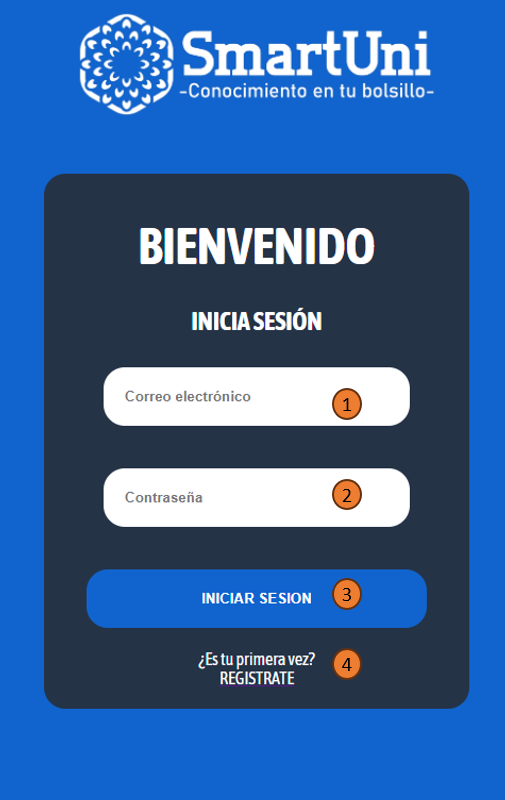
\includegraphics[scale = 0.5]{1.png}
    \caption{Inicio}
    \label{fig:Figura3.4.3}
\end{figure}

\section{Registro}
Una vez pulsado registrarse en la página de bienvenida será redirigido aquí, donde rellenando los campos podrás crear su cuenta para disfrutar de los servicios de la aplicación.
\\Para crear su cuenta deberá rellenar todos los campos con tu información de la cuenta a crear. en el campo de correo electrónico (1) deberá insertar el correo electrónico al que desea vincular su cuenta, seguido de esto deberá escribir su contraseña en el campo (2) y (3) para verificar que no se ha equivocado a la hora de escribir la contraseña, una vez rellenados esos datos podrá pulsar el botón de registrarse (4) y se le redirigirá al menú B.3, en caso de haber entrado a esta página por error, si ya tiene una cuenta podrá pulsar el botón de iniciar sesión (5), lo que le devolverá a la pagina de bienvenida B.1.
\begin{figure}[H]
    \centering
    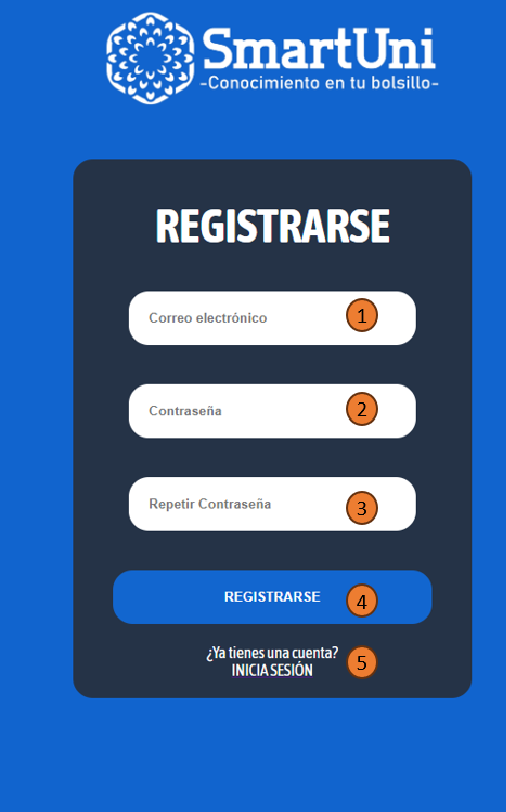
\includegraphics[scale = 0.5]{3.png}
    \caption{Registrarse}
    \label{fig:Figura3.4.3}
\end{figure}

\section{Menú}
El menú muestra las diferentes secciones del programa a las que puede acceder, el botón (1) le redirigirá al listado de las aulas,B.4, donde podrá ver las diferentes aulas del centro y que se imparte en ellas, el botón (2) le redirigirá a su taquilla, B.8, si posee una o al listado de taquillas, B.6, donde podrá reservar una para uso personal, el botón (3) le llevará a la sección de cafetería, B.9, donde podrá realizar un pedido de manera remota para poder recogerlo y disfrutar de la comida de la cafetería. Si quiere salir de la aplicación podrá pulsar el botón cerrar sesión (4).
\begin{figure}[H]
    \centering
    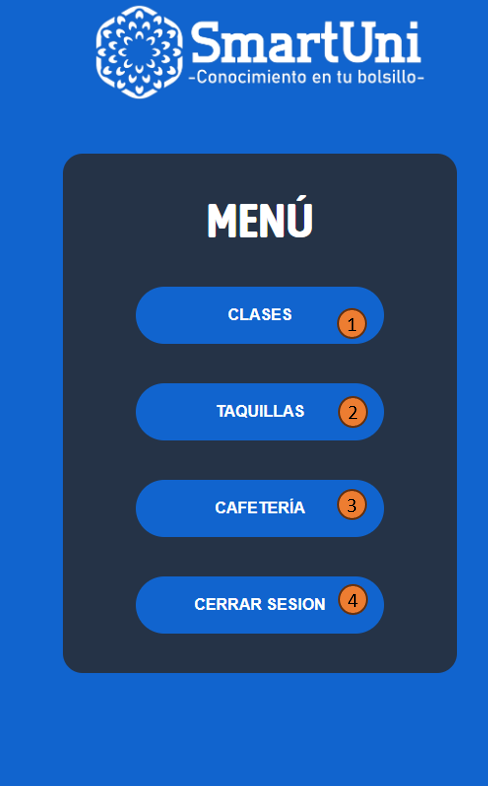
\includegraphics[scale = 0.5]{2.png}
    \caption{Menú}
    \label{fig:Figura3.4.3}
\end{figure}

\section{Listado de aulas}
Esta página muestra un listado dentro del Box(2) de todas las aulas de las que se dispone información, para ver en detalle la información del aula deberá pulsar el botón del aula que desee(3). En caso de querer volver al menú, podrá pulsar la imagen de SmartUni de la parte superior de la pantalla(1).
\begin{figure}[H]
    \centering
    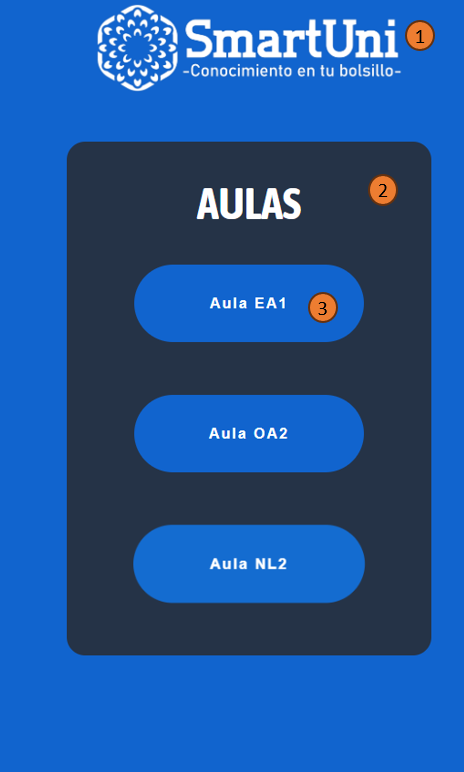
\includegraphics[scale = 0.5]{4.png}
    \caption{Listado de aulas}
    \label{fig:Figura3.4.3}
\end{figure}

\section{Detalle de un aula}
En esta página se detallará la información disponible sobre el aula, como puede ser la temperatura o las asignaturas que se imparten en ella junto a sus horarios. En caso de querer volver al menú, podrá pulsar la imagen de SmartUni de la parte superior de la pantalla(1).
\begin{figure}[H]
    \centering
    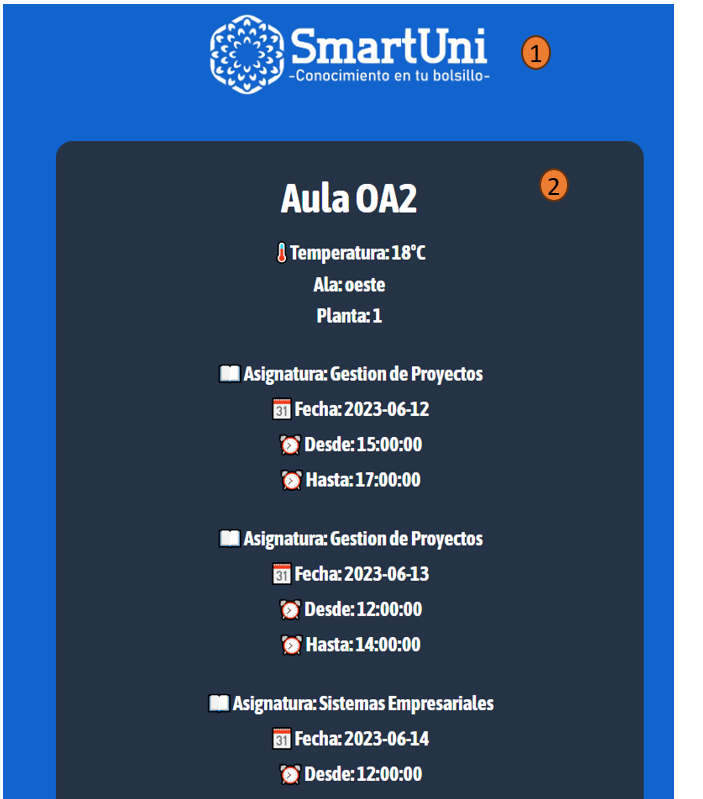
\includegraphics[scale = 0.5]{5.png}
    \caption{Detalle de un aula}
    \label{fig:Figura3.4.3}
\end{figure}

\section{Listado de taquillas}
Esta página muestra un listado dentro del Box(2) de todas las taquillas disponibles, para ver en detalle la información de la taquilla deberá pulsar el botón de la taquilla que desee(3). En caso de querer volver al menú, podrá pulsar la imagen de SmartUni de la parte superior de la pantalla(1).
\begin{figure}[H]
    \centering
    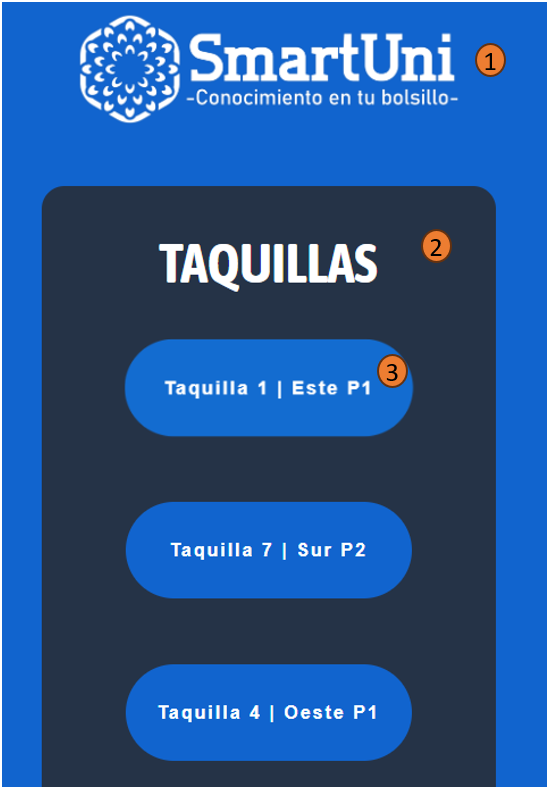
\includegraphics[scale = 0.5]{6.png}
    \caption{Listado de taquillas}
    \label{fig:enter-label}
\end{figure}

\section{Reserva de Taquilla}

En esta página se ve la información disponible de la taquilla(2), también se puede ver el botón de solicitar taquilla(3), que al pulsarlo le dirigirá a B.7 y vinculará la taquilla a su usuario. En caso de querer volver al menú, podrá pulsar la imagen de SmartUni de la parte superior de la pantalla(1).
\begin{figure}[H]
    \centering
    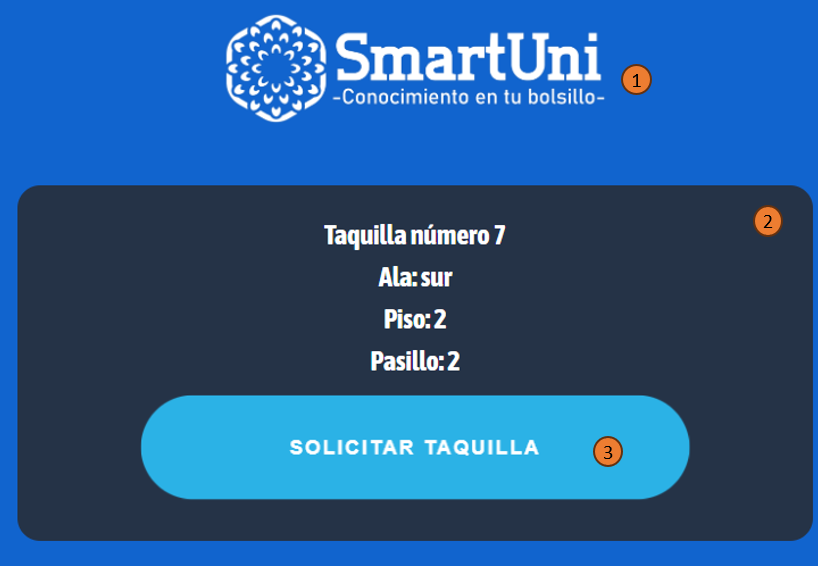
\includegraphics[scale = 0.5]{8.png}
    \caption{Reservar una taquilla}
    \label{fig:Figura3.4.3}
\end{figure}

\section{Taquilla reservada}
Una vez reservada la taquilla podremos acceder a esta página en la que se mostrará la información de la taquilla incluyendo la contraseña con la que podrá abrir la taquilla pertinente, se dispone de el botón de cancelar taquilla(3), que desvinculará la cuenta de la taquilla. En caso de querer volver al menú, podrá pulsar la imagen de SmartUni de la parte superior de la pantalla(1).
\begin{figure}[H]
    \centering
    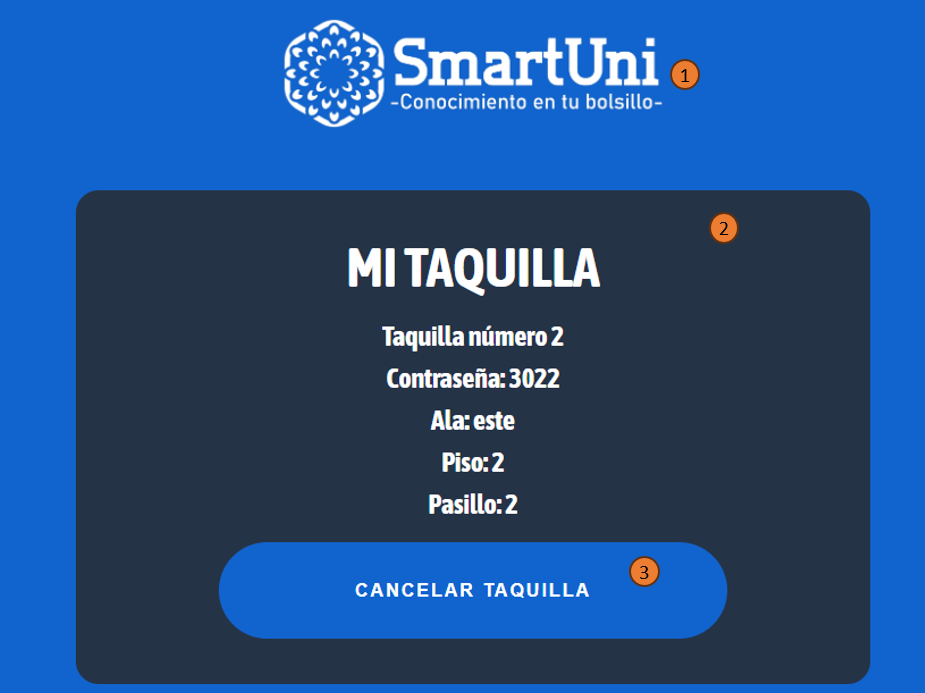
\includegraphics[scale = 0.5]{7.png}
    \caption{Detalle de una taquilla}
    \label{fig:enter-label}
\end{figure}

\section{Inicio de cafetería}
Esta pagina representa el inicio de la cafetería, en ella se puede realizar un pedido(2), pulsando este botón accederá a B.10. O acceder a los pedidos que ya ha realizado(3), que le redirigirá a B.11. En caso de querer volver al menú, podrá pulsar la imagen de SmartUni de la parte superior de la pantalla(1).
\begin{figure}[H]
    \centering
    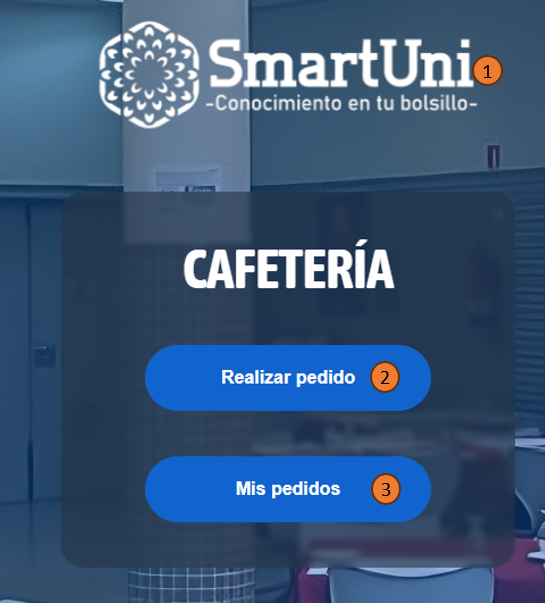
\includegraphics[scale = 0.5]{9.png}
    \caption{Inicio de la cafetería}
    \label{fig:enter-label}
\end{figure}

\section{Realizar Pedido}
En esta página podrá realizar su pedido de la cafetería, en ella dispone de información como recomendaciones generales y personalizadas(2). también dispondrá de un buscador en el que podrá filtrar los productos por su nombre(3). Para seleccionar sus productos dispone de un listado de botones(5) con los cuales podrá rellenar su pedido. Cada producto esta relacionado a 3 botones, el principal que es el central(7) mostrará la información del producto junto con una foto de el, el botón de +(8), que añadirá una unidad del producto seleccionado a la cesta de compra, y el botón -(6), que quitará una unidad del producto seleccionado a la cesta de compra. En caso de querer volver al menú, podrá pulsar la imagen de SmartUni de la parte superior de la pantalla(1).
\begin{figure}[H]
    \centering
    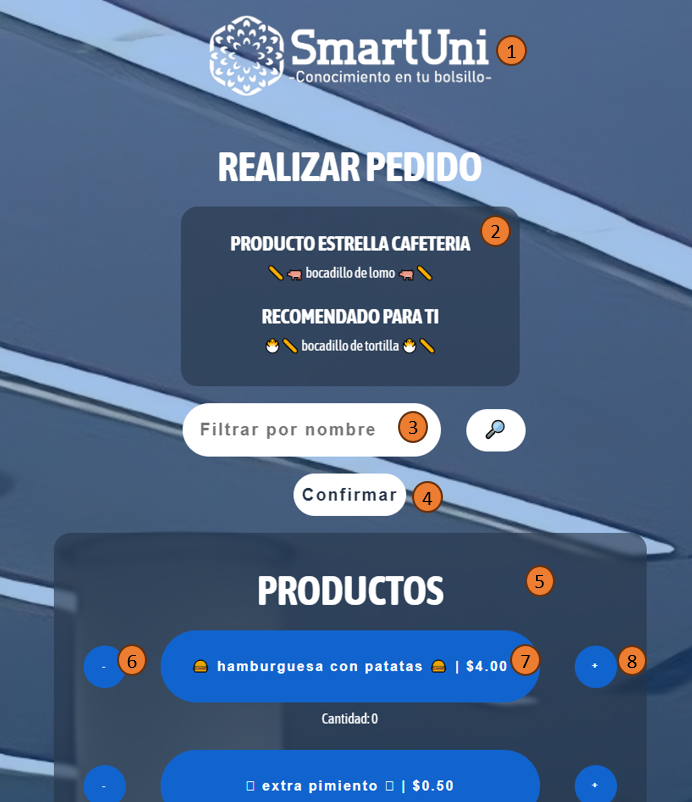
\includegraphics[scale = 0.5]{10.png}
    \caption{Realizar pedido}
    \label{fig:enter-label}
\end{figure}

\section{Seleccionar pedido}
En esta pagina podrá ver los diferentes pedidos que haya realizado(2), al pulsar en su pedido(3), se le redirigirá a B.12. Los pedidos marcados en rojo son pedidos ya finalizados o cancelados. En caso de querer volver al menú, podrá pulsar la imagen de SmartUni de la parte superior de la pantalla(1).
\begin{figure}[H]
    \centering
    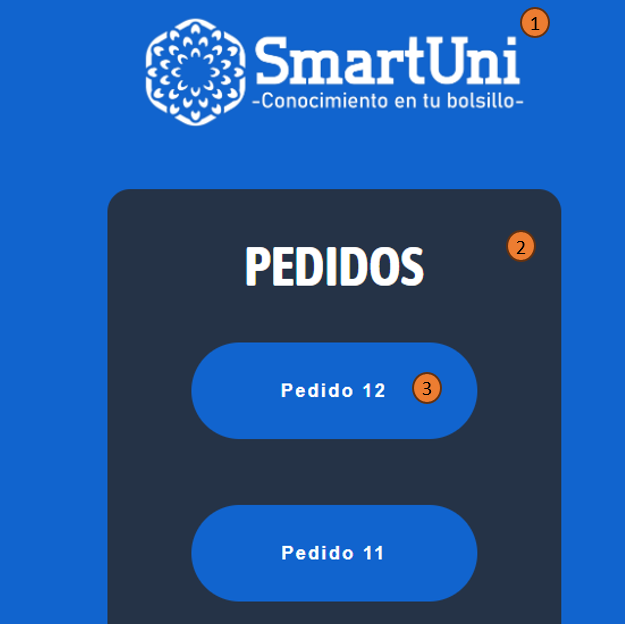
\includegraphics[scale = 0.5]{12.png}
    \caption{Seleccionar pedido}
    \label{fig:enter-label}
\end{figure}

\section{Información de un pedido}
Esta pagina muestra la información de el pedido seleccionado(2), en ella además se podrá escanear el NFC (3)correspondiente a su pedido, la información sobre este NFC se dispondrá en el momento en que se asocie el pedido a una bandeja. En caso de querer volver al menú, podrá pulsar la imagen de SmartUni de la parte superior de la pantalla(1). Así como poder simularlo(4), este botón simulara la conexión con el NFC de manera ficticia.
\begin{figure}[H]
    \centering
    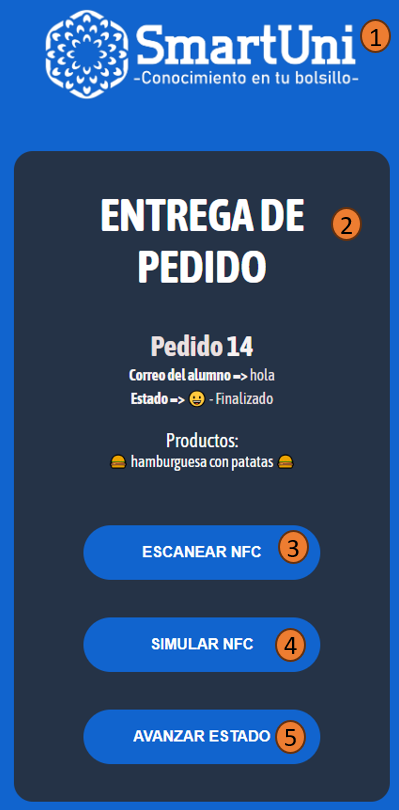
\includegraphics[scale = 0.5]{11.png}
    \caption{Información de un pedido}
    \label{fig:enter-label}
\end{figure}


\newpage
\chapter{Simulación de datos}

\newpage
\chapter{Hojas de características de los componentes}

\newpage
\end{appendices}
% \chapter{Marco teórico}
% \section{Computación ubicua}
% \lipsum[1-2]
% \newpage
% \section{Internet de las cosas}
% \lipsum[3-4]
% \newpage
% \section{Universidad de Alcalá}
% \lipsum[5-6]

% \chapter{Metodología}
% \section{Desarrollo del proyecto}
% \lipsum[1-2]
% \newpage
% \section{Etapas del proyecto}
% \lipsum[3-4]

% \chapter{Resultados}
% \section{Análisis de los resultados}
% \lipsum[1-2]
% \newpage
% \section{Discusión de los resultados}
% \lipsum[3-4]

% \chapter{Conclusiones}
% \section{Logros alcanzados}
% \lipsum[1-2]
% \newpage
% \section{Recomendaciones}
% \lipsum[3-4]
% \newpage
% \section{Trabajo futuro}
% \lipsum[5-6]

\end{document}
